\documentclass[a4paper,11pt]{article}
%\textwidth 11,8 cm
%\textheight 17 cm
\textheight 23 cm
\topmargin -10mm
%\usepackage{graphicx}
\usepackage{amsmath}
\usepackage{amsfonts}
\usepackage{amssymb}
\usepackage{eufrak}
\usepackage{stmaryrd}
\usepackage{makeidx}
\usepackage{times}
%\usepackage{mathptmx}
%Uncomment next line for pdflatex and use includegraphics with eps file
% for latex2html don't use the option [width=\textwidth]
% check that xfig files are exported magnif 100%

 \usepackage[ps2pdf,
            breaklinks=true,
            colorlinks=true,
            linkcolor=red,
            citecolor=green
            ]{hyperref}

%HEVEA\htmlfoot{Retour \`a la page personnelle de \ahref{http://www-fourier.ujf-grenoble.fr/\~parisse}{Bernard Parisse}.}
%HEVEA\htmlhead{Retour \`a la page personnelle de \ahref{http://www-fourier.ujf-grenoble.fr/\~parisse}{Bernard Parisse}.}
\usepackage{pst-plot}
\usepackage{graphicx}

%\def\@evenhead{\thepage\hfill{\footnotesize\textit{\leftmark}}}
%\def\@oddhead{\footnotesize{\textit{\rightmark}}\hfill\thepage}
%\usepackage{hp}
%HEVEA\@def@charset{US-ASCII}
\usepackage[utf8]{inputenc}
\usepackage[T1]{fontenc}
\usepackage[francais]{babel}
\usepackage{latexsym}

\newcommand{\R}{{\mathbb{R}}}
\newcommand{\C}{{\mathbb{C}}}
\newcommand{\Z}{{\mathbb{Z}}}
\newcommand{\N}{{\mathbb{N}}}
%\usepackage[pdftex]{hyperref}
\title {L'interface {\tt Xcas} de {\tt giac}}
\author{Ren\'ee De Graeve\\ Ma\^itre de Conf\'erence \`a Grenoble I}
\date{}
\makeindex
\begin{document}
\newcommand{\asinh}{\,\,\mbox{asinh\,}}
\newcommand{\atanh}{\,\,\mbox{atanh\,}}
\maketitle


\vfill
{\bf \centerline{Remerciements}}
Je  remercie:
 \begin{itemize}
\item Bernard Parisse pour ses pr\'ecieux conseils et ses remarques sur ce texte,

 \end{itemize}

\vspace{1cm}


\copyright\ 2002, 2006 Ren\'ee De Graeve, \verb|renee.degraeve@wanadoo.fr|\\
La copie, la traduction et la redistribution de ce document sur
support \'electronique
ou papier sont autoris\'es pour un usage non commercial uniquement.
L'utilisation de ce document \`a des fins commerciales est interdite
sans l'accord \'ecrit du d\'etenteur du copyright.
Cette documentation est fournie en l'\'etat, sans garantie d'aucune
sorte. En aucun cas le d\'etenteur du copyright ne pourra \^etre tenu
pour responsable de dommages r\'esultant de l'utilisation de ce
document.
\newpage
\printindex
\newpage
\tableofcontents
\newpage 
\section*{Pr\'eambule}
{\tt giac} est la biblioth\`eque C++ de fonctions de calcul formel que l'on 
peut utiliser  avec plusieurs interfaces dont {\tt Xcas}.\\
On d\'etaille ici l'interface  {\tt Xcas}, pour les autres utilisations de 
{\tt giac} se reporter au d\'ebut du manuel de Calcul formel (menu 
{\tt Aide -> Manuels}).
\subsection{Notations}
Lorsque l'on doit appuyer sur 2 touches en m\^eme temps on reliera ces deux 
touches avec  {\tt +}. Par exemple, si on doit appuyer en m\^eme temps sur
{\tt Alt} et sur {\tt t} on \'ecrira {\tt Alt+t}.

Lorsque l'on veut indiquer le choix \`a faire dans un menu on reliera les 
diff\'erents sous-menus avec $\blacktriangleright$ : on \'ecrira par exemple
{\tt Expression}$\blacktriangleright${\tt factor} pour dire que la commande 
{\tt factor} se trouve dans le menu {\tt Expression}.
\section{Pour commencer}
\subsection{Le principe}
L'interface  {\tt Xcas} va vous permettre d'ouvrir plusieurs sessions de 
calculs : chaque session utilise la m\^eme barre de menus (appel\'ee dans la  
suite "barre du menu g\'en\'eral" : {\tt Fich, Edit, Cfg...}), et chaque 
session peut (ou non) \^etre sauv\'ee. Les noms des diff\'erentes sessions (ou 
{\tt Unammed}) s'inscrivent dans la ligne situ\'ee sous cette 
barre de menus et le nom de la session active est en surbrillance. 

Ces sessions ont plusieurs niveaux 
d'entr\'ee, sont ind\'ependantes les unes des autres 
et on peut passer de l'une \`a l'autre en cliquant sur son nom.

Chaque session a une ligne de boutons qui lui est propre :
\begin{itemize}
\item \framebox{\tt ?} pour ouvrir le sous menu {\tt Index} 
du menu {\tt Aide} : si on tape le d\'ebut d'une commande puis \framebox{\tt ?}
dans une ligne de commandes cela ouvre le menu {\tt Aide} \`a l'endroit 
indiqu\'e par ce d\'ebut.
\item  \framebox{\tt Save} pour sauver la session 
%(par exemple sous le nom  {\tt essai.xws}). \framebox{\tt Save} est sur fond vert si on la session a \'et\'e sauv\'ee et sinon \framebox{\tt Save} est sur fond rose,
\item \framebox{\tt Config : exact real RAD 12 xcas 12.65M} pour configurer la 
session : c'est le bouton "ligne d'\'etat" qui rappelle la configuration 
choisie.  
%On appelera ce bouton "ligne d'\'etat". On notera que lorsque l'on a sauv\'e la session par exemple sous le nom  {\tt essai.xws} cette ligne devient :\\\framebox{\tt Config essai.xws : exact real RAD 12 xcas 12.65M}.
\item \framebox{\tt STOP} pour arr\^eter un calcul trop long il faut cliquer sur
\framebox{\tt STOP}. Il faut 
quelquefois taper \`a la fois sur {\tt SHIFT} de votre clavier et cliquer sur 
\framebox{\tt STOP} pour que le calcul s'arr\^ete.\\
{\bf Attention} Si vous \^etes en train de faire des calculs dans d'autres 
sessions, \framebox{\tt STOP} va arr\^eter tous ces calculs. Pour \'eviter 
cela, vous pouvez faire  \framebox{\tt Shift+STOP} cela tuera seulement la 
tache de la session visible ....mais cela est plus brutal et pour ne pas avoir 
de probl\`emes ult\'erieurement, il faut ensuite tout sauver et relancer 
{\tt Xcas}.
\end{itemize}

Chaque session est compos\'ee de niveaux num\'erot\'es qui peuvent \^etre de 
diff\'erentes natures~: ligne de commandes pour le calcul formel, 
g\'eom\'etrie dynamique et formelle, tableur formel, dessin tortue etc... 

Au sein d'une m\^eme session, les  diff\'erents niveaux d'entr\'ee ne sont pas 
ind\'ependants, par exemple, une variable d\'efinie dans une ligne de commandes
pourra \^etre utilis\'ee en g\'eom\'etrie ou dans le tableur.
L'ensemble de toutes ces sessions constitue votre espace de travail.

\subsection{Le d\'emarrage}
Pour ouvrir un espace de travail, on clique sur l'ic\^one {\tt xcasfr} du 
bureau sous Windows ou de Applications sur Mac OS X ou du menu Education
(Linux/Gnome) ou on tape dans un terminal sous Linux : {\tt xcas \&}

La premi\`ere fois que vous lancez {\tt Xcas}, 
on vous demandera le premier niveau que vous voulez avoir au d\'emarrage, \`a 
choisir parmi~:
\begin{center}
{\tt \framebox{Autres} \framebox{Xcas} \framebox{Maple} }
\end{center}
afin d'avoir toujours le m\^eme environnement \`a chaque d\'emarrage.
\begin{itemize}
\item Si vous tapez sur {\tt Enter} ou sur {\tt Xcas} c'est 
la syntaxe {\tt Xcas} qui sera s\'electionn\'ee. 
\item Si vous cliquez sur {\tt Maple} c'est 
la syntaxe {\tt Maple} qui sera s\'electionn\'ee. 
\item Si vous cliquez sur {\tt Autres}, vous devrez choisir 
entre {\tt Geometrie}, {\tt Tableur} et {\tt Tortue}. \\
Ainsi si vous cliquez sur {\tt Tortue}, 
un niveau de programme et un dessin {\tt Tortue} 
seront lanc\'es au d\'emarrage.
\end{itemize}
Ce choix n'influe que sur l'\'ecran que l'on obtient au 
d\'emarrage car \`a tout moment vous pouvez cr\'eer un nouveau niveau 
d'entr\'ee de n'importe quelle nature et \`a n'importe quel endroit de votre 
session ou encore ouvrir une nouvelle session. Vous pouvez changer 
ult\'erieurement de mode de d\'emarrage (menu {\tt Cfg} puis 
{\tt Configuration generale}, on valide son choix, puis menu  {\tt Cfg} et 
{\tt Sauver preferences}) ou de syntaxe (bouton de configuration 
{\tt Config:...}).

Vous pouvez aussi relancer l'\'ecran initial de configuration 
en effa\c{c}ant le fichier :
\verb|~/.xcasrc| sous Linux ou {\tt xcas.rc} sous Windows.

\subsection{Un premier calcul}\label{sec:calc}
On suppose qu'au d\'emarrage vous avez choisi {\tt Xcas} ou que vous avez 
cr\'e\'e une ligne de commandes en tapant {\tt Alt+n}.\\
Si on veut  utiliser une commande de {\tt Xcas}, il suffit de la taper
dans une ligne de commandes puis de valider avec la touche {\tt Enter}.\\
{\bf Attention!!!!} Dans la suite {\tt Enter} sera sous-entendu.\\
On tape par exemple :
\begin{center}
{\tt 1+2}
\end{center}
On obtient :
\begin{itemize}
\item en dessous la r\'eponse {\tt 3} dans un \'editeur d\'equations,
\item la cr\'eation d'un niveau de num\'ero 2. 
\end{itemize}
\noindent On tape~:
\begin{center}
{\tt 100!}
\end{center}
On obtient :
\begin{itemize}
\item la r\'eponse dans un \'editeur d'expressions poss\'edant une  barre de 
scroll horizontale  situ\'ee  sous la r\'eponse qui permet de lire la valeur 
exacte de 100!,
\item la cr\'eation d'un niveau de num\'ero 3. 
\end{itemize}
\ \\
\noindent On tape maintenant~:
\begin{center}
{\tt expand((1+x)\verb|^|90)}
\end{center}
On obtient :
\begin{itemize}
\item la r\'eponse dans un \'editeur d\'equations poss\'edant une  barre de 
scroll horizontale situ\'ee  sous le r\'eponse et une  barre de scroll 
verticale situ\'ee \`a droite de la r\'eponse qui permet de lire le 
r\'esultat,
\item la cr\'eation d'un niveau de num\'ero 4, 
\item la cr\'eation d'une barre de scroll verticale pour la session situ\'ee 
\`a droite de la barre de scroll verticale permettant de lire le 
d\'eveloppement de $(1+x)^{90}$.
\end{itemize}
\begin{center}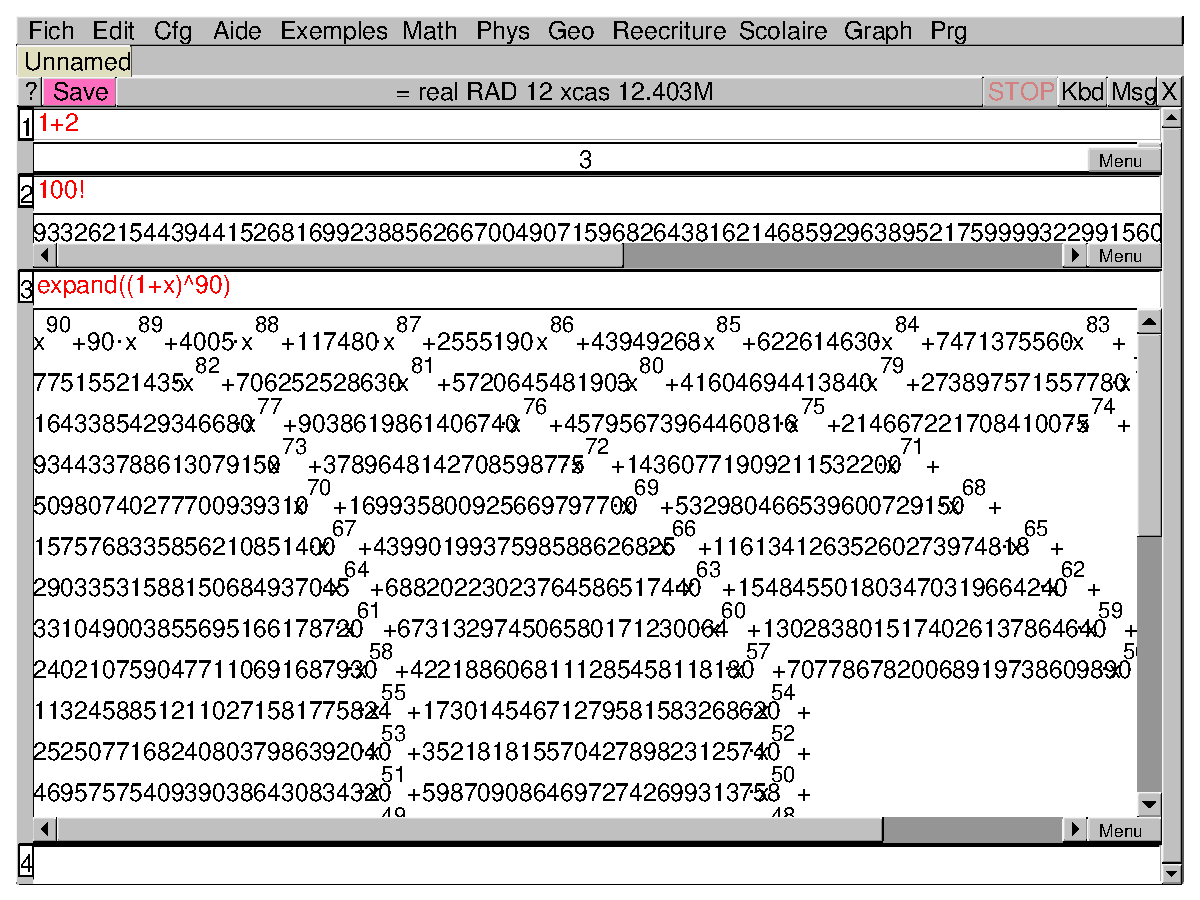
\includegraphics[width=12.5cm]{windowinter}\end{center}
{\bf Remarques}~:
\begin{itemize}
\item Si vous avez choisi {\tt expand} \`a partir du  
menu {\tt Expression $\blacktriangleright$Rationnel} une aide succincte sur 
{\tt expand} s'affiche dans la ligne des messages (touche {\tt msg} du clavier 
obtenu avec le bouton {\tt Kbd}), et si dans la configuration g\'en\'erale vous
avez coch\'e {\tt Aide HTML auto} une aide plus compl\`ete peut
s'afficher dans le navigateur (par d\'efaut sous Linux c'est Mozilla  et
par d\'efaut sous Windows c'est le navigateur int\'egr\'e).
Par contre, si vous avez cliqu\'e sur {\tt expand} dans le 
bandeau (obtenu en cliquant sur {\tt cmds} du clavier{\tt Kbd}), seule l'aide 
succincte apparait. 
Pour voir ce bandeau il faut avoir choisi 
{\tt Cfg$\blacktriangleright$Montrer$\blacktriangleright$Bandeau}, 
ou en cliquant sur la touche {\tt cmds} du clavier obtenu avec le bouton
{\tt Kbd}. {\tt expand} se trouve en cliquant sur {\tt Expression} puis sur 
{\tt Rationnel}.
 \item Si le temps de calcul est sup\'erieur \`a
0.1s, ce temps s'affiche en bleu dans la zone interm\'ediaire
reserv\'ee aux affichages de programmes.
\end{itemize}

\subsection{Les niveaux}
Les niveaux sont constitu\'es :
\begin{itemize}
\item soit une ligne de commandes : dans cette ligne on tape des commandes de 
{\tt Xcas} separ\'ees par {\tt ;} ou par {\tt ,} et on les ex\'ecute en tapant 
{\tt Enter}. Il apparait alors un emplacement pour les affichages 
interm\'ediaires (si il y en a) 
%des instructions {\tt print} dans la commande) 
et un emplacement pour la r\'eponse qui peut \^etre, selon la nature de la 
commande, un \'editeur d'expressions ou une fen\^etre graphique. 
%(identique \`a une figure de g\'eom\'etrie en mode {\tt Rep\`ere}).
Lorsqu'on met dans la m\^eme ligne de commandes, plusieurs commandes separ\'ees
par une virgule ou un point virgule, c'est la nature de la derni\`ere commande 
qui d\'etermine la nature de la sortie. On peut par exemple\'ecrire :
\begin{center}{\tt carre(0,1),0}\end{center} 
pour ne pas avoir une sortie graphique mais pour avoir une sortie texte. La 
r\'eponse donnera alors la liste des coordonn\'ees des sommets du carr\'e.
On pourra remarquer que l'\'ecran d'une sortie graphique est identique \`a une 
figure de g\'eom\'etrie en mode {\tt Rep\`ere}.
\item soit un \'editeur d'expressions ou d'expressions, qui permet de saisir 
des expressions math\'ematiques en affichage 2-d c'est \`a dire sans 
parenth\`eses (cf. la section \ref{sec:eqw}),
\item soit un niveau de g\'eom\'etrie 2-d, son \'ecran, ses menus et boutons 
et ses lignes de  commandes,
\item soit un niveau de g\'eom\'etrie 3-d, son \'ecran, ses menus et boutons 
et ses lignes de commandes,
\item soit un niveau de dessin tortue (logo), son \'ecran, son \'editeur de 
programmes, ses menus et boutons et ses lignes de commandes,
\item soit un tableur, ses menus, ses boutons et son \'ecran graphique 2-d,
\item soit un \'editeur de programmes, ses menus et boutons,
\item soit un commentaire,
\item soit un regroupement de ces niveaux en un groupe.
\end{itemize}
Le niveau actif est celui o\`u se trouve le curseur et le niveau 
s\'electionn\'e est obtenu quand on clique sur son num\'ero, num\'ero qui 
s'\'ecrit alors sur fond noir.

On peut effacer ou d\'eplacer un niveau ou un groupe de niveaux
dans une session, ou encore le recopier dans une autre session.
On peut \`a tout moment ins\'erer un nouveau niveau  ou un groupe de niveaux
ou encore modifier l'entr\'ee d'un niveau : {\tt Enter} valide alors le 
changement de commandes de ce niveau et positionne le curseur sur l'entr\'ee 
suivante, mais les niveaux suivants ne seront pas recalcul\'es. Il est 
toutefois possible apr\`es une modification de r\'eex\'ecuter, soit tous les 
niveaux, soit les niveaux situ\'es apr\`es la modification (menu {\tt Edit} 
puis {\tt Executer session}  ou {\tt Executer en\_dessous}).

{\bf Remarques}\\
Dans une figure de g\'eom\'etrie, il est important de revalider les commandes,
apr\`es toutes modifications, d\`es le premier niveau modifi\'e car dans une 
figure de g\'eom\'etrie, la validation d'un niveau entraine la validation des 
niveaux suivants sauf si on a cliqu\'e sur {\tt Step}.

\section{Votre espace de travail}\index{F1}\index{F9}\index{Tab}\index{?}
Vous obtenez au d\'emarrage une session avec de haut en bas~:
\begin{enumerate}
\item La barre du menu g\'en\'eral {\tt Fich Edit Cfg... Phys Scolaire Tortue} 
contenant les fonctions de {\tt Xcas} et ce qu'il faut pour les configurer et 
pour sauver ou charger une session de travail.
\item Une ligne des noms de sessions qui contiendra les noms (ou {\tt Unnamed} 
si elles n'ont pas de noms) de vos diff\'erentes sessions. Au d\'emarrage il 
n'y a qu'une session qui n'a pas de nom donc sur cette ligne il y a 
{\tt Unnamed},
\item Un bandeau g\'en\'eral avec de gauche \`a droite :
\begin{itemize}
\item Un bouton \framebox{\tt ?} permettant d'ouvrir le sous menu {\tt Index} 
du menu {\tt Aide}. Il faut savoir que si on tape
le d\'ebut d'une commande puis le bouton \framebox{\tt ?} (ou la touche de 
tabulation ou sur la touche \framebox{F1} de v\^otre ordinateur)
dans une ligne de commandes cela ouvre le menu {\tt Aide} \`a l'endroit 
indiqu\'e par ce d\'ebut. Par contre, dans l'\'editeur de programmes le bouton 
\framebox{\tt ?} (ou  la touche \framebox{F1} de v\^otre ordinateur) permettent
d'ouvrir le sous menu {\tt Index} du menu {\tt Aide} alors que la touche de 
tabulation de v\^otre ordinateur sert  \`a indenter l'\'ecriture d'un programme.
\item Un bouton \framebox{\tt Save}, sur fond rose, servant \`a sauver votre 
session en lui donnant un nom par exemple {\tt session1.xws}. Quand la session 
a \'et\'e sauv\'e le fond du bouton \framebox{\tt Save} devient vert et
{\tt Unnamed} est remplac\'e par le nom de fichier, par exemple par
{\tt session1.xws}. Notez que
les noms des sessions ont comme extension {\tt .xws} et cette extension est 
rajout\'ee automatiquement si vous l'avez oubli\'ee.
\item Un bouton \framebox{\tt Config : exact real RAD 12 xcas 12.65M} ou\\
 \framebox{\tt Config essai.xws : exact real RAD 12 xcas 12.65M} si on a sauv\'e la 
session sous le nom  {\tt essai.xws}.\\
Ce  bouton "ligne d'\'etat" ouvre la fen\^etre permettant de configurer 
le CAS et sur lequel est marqu\'e la ligne d'\'etat rappelant cette 
configuration., dans l'exemple, on 
est en mode exact et r\'eel, les angles sont exprim\'es 
en radian, les calculs num\'eriques sont faits avec 12 chiffres 
significatifs, le style de programmation est {\tt xcas} et enfin les 
resources en m\'emoire demand\'ees par le calcul sont de 12.65M (c'est la 
taille m\'emoire en M\'egabits utilis\'ee par {\tt Xcas}).\\
Sur cette ligne d'\'etat, le mode num\'erique sera not\'e {\tt approx} et le 
mode complexe sera not\'e :
\begin{itemize}
\item {\tt cplx} si les variables ne sont pas consid\'er\'ees comme complexes 
(on a alors {\tt re(z)=z} et {\tt conj(z)=z}), 
\item {\tt CPLX} si les variables sont consid\'er\'ees comme complexes 
(on a alors {\tt re(z)=re(z)} et {\tt im(z)=im(z)} qui seront not\'es
respectivement  $\mathfrak R(z)$ et $\mathfrak I(z)$ dans la r\'eponse).
\end{itemize}
Notez que ce bouton "ligne d'\'etat"  ouvre la fen\^etre de 
configuration qui est aussi obtenue \`a partir du menu :
{\tt Cfg$\blacktriangleright$Configuration du CAS},
\item  Un bouton rouge \framebox{\tt STOP} pour arr\^eter un calcul trop long, 
{\bf Attention} Si vous \^etes en train de faire des calculs dans d'autres 
sessions, \framebox{\tt STOP} va arr\^eter tous ces calculs. Pour \'eviter 
cela, vous pouvez faire  \framebox{\tt Shift+STOP} cela tuera seulement la 
t\^ache de la session visible ....mais cela est plus brutal et pour ne pas 
avoir de probl\`emes ult\'erieurement, il faut ensuite tout sauver et relancer 
{\tt Xcas}.
\item Un bouton \framebox{\tt Kbd}, servant \`a faire apparaitre ou disparaitre
un clavier scientifique.
On remarquera sur ce clavier :
\begin{itemize}
\item la touche \framebox{\tt cmds} qui sert \`a faire apparaitre
ou disparaitre une barre de boutons contenant les commandes du CAS, appel\'ee 
bandeau du CAS. Dans le bandeau, on remarquera la touche {\tt kbd} qui sert 
\`a faire apparaitre ou disparaitre le clavier.
\item la touche \framebox{\tt msg}, servant \`a faire apparaitre
 ou disparaitre une fen\^etre de messages facilement lisible gr\^ace \`a sa 
barre de scroll. Cette fen\^etre vous donne des messages comme
{\bf Success} pour dire que tout s'est bien pass\'e, ou affiche une aide 
succinte sur la commande choisie \`a partir du menu g\'en\'eral, ou ce qu'il 
faut ins\'erer dans votre fichier \LaTeX  pour ins\'erer la figure sauv\'ee, 
par exemple, sous le nom {\tt session1.eps} :
\begin{center}{\bf Use }\verb|\includegraphics[width=\textwidth]{session1}|\end{center} 
\begin{center}{\bf inside your latex document, with header }\verb|\usepackage{graphicx}|\end{center}  
\item la touche \framebox{\tt abc}, servant \`a faire apparaitre ou disparaitre
un clavier contenant les lettres en minuscule, par ordre alphab\'etique, ainsi 
que des signes de ponctuation. On notera qu'en appuyant sur la touche 
{\tt $\alpha$} on obtient un clavier contenant les lettres grecques et qu'en 
appuyant sur la touche  {\tt Maj} transforme le clavier avec des lettres en 
majuscule.
\item  la touche \framebox{\tt$\blacktriangleleft$ } qui permet de supprimer ce que l'on a s\'electionn\'e,
\item  la touche \framebox{\tt coller} qui permet de recopier ce que 
l'on a s\'electionn\'e, 
\item   la touche verte \framebox{\tt $\hookleftarrow$} qui sert de touche 
{\tt Enter}.
\item   la touche \framebox{ $\vartimes$} situ\'e tout en haut \`a 
droite, permettant de faire disparaitre le clavier {\tt Kbd}.
\end{itemize}
\item Un bouton \framebox{ $\vartimes$} situ\'e tout \`a 
droite, permettant de fermer la session en cours. 
Cela provoquera \'eventuellement 
un avertissement si les derni\`eres modifications n'ont pas \'et\'e sauv\'ees.
\end{itemize} 
\item Un premier niveau ou les deux premiers niveaux, selon le  d\'emarrage 
choisi.\\
Si au d\'emarrage, on a choisi : 
\begin{itemize}
\item {\tt Xcas},\\
le premier niveau (de num\'ero 1) est un niveau "ligne de commandes" 
c'est \`a dire une ligne pour taper des commandes de {\tt Xcas}.\\
La r\'eponse \`a une commande non graphique se marque dans un \'editeur 
d'\'equations. On pourra ainsi facilement re\'ecrire diff\'eremment cette 
r\'eponse ou une partie de cette r\'eponse. Pour cela, il suffit de 
s\'electionner la r\'eponse ou une partie de cette r\'eponse et de 
s\'electionner dans le  menu {\tt Expression}, la commande qui permet cette 
re\'ecriture. Pour que la r\'eponse soit plus lisible, la multiplication
$\ast$ sera not\'e avec une toute petite \'etoile ({\tt *}) ressemblant \`a 
un point.\\
Remarquez le petit bouton {\tt M} \index{M}
situ\'e en bas et \`a droite de cet \'editeur d'expressions. 
Ce  bouton {\tt M} permet avec :
\begin{itemize}
\item {\tt Selectionner tout}, de recopier ce qui se trouve dans 
l'\'editeur d'un seul clic,
\item {\tt Eval selection}, d'\'evaluer la s\'election, 
\item {\tt Evalf selection}, d'\'evaluer numeriquement la s\'election, 
\item {\tt Arriere}, de se d\'eplacer en arri\`ere, dans l'historique de 
l'\'editeur d'expressions, et de retrouver la r\'eponse initiale dans le cas 
o\`u, on a fait une modification malencontreuse, 
\item {\tt Avant}, de se d\'eplacer en avant, dans l'historique de l'\'editeur 
d'\'equations, 
%et de revenir \`a la r\'eponse d'avant dans le cas o\`u on aurait utilis\'e trop de fois l'item {\tt Arriere}.
\end{itemize}
\item {\tt Tortue}, \\
le premier niveau sera un niveau "dessin tortue" avec :\\
\`a gauche, une ligne de commandes de num\'ero 1,\\ 
 au centre, un \'ecran graphique  pour piloter la tortue et\\ 
\`a droite, un \'ecran pour le r\'ecapitulatif des commandes~;\\
le deuxi\`eme niveau sera un niveau "\'editeur de programmes" c'est \`a dire 
un \'editeur pour taper des programmes et sa barre de menu.
\end{itemize}
\item Selon la configuration, un clavier virtuel (que l'on peut faire 
apparaitre ou disparaitre en appuyant sur \framebox{\tt Kbd}) ou rien,
\end{enumerate}


\section{La barre du menu g\'en\'eral}
En haut de votre \'ecran, vous voyez :\\
%{\tt Fich Edit Cfg Aide CAS Tableur Graphic Geo}\\
%{\tt Prg Expression Cmds Phys Scolaire Tortue}
{\tt Fich Edit Cfg Aide CAS Expression Cmds Prg }\\
{\tt Graphic Geo Tableur Phys Scolaire Tortue}

\subsection{Le menu {\tt Fich}}
\begin{itemize}
\item
{\tt Nouvelle session}  pour cr\'eer et ouvrir une nouvelle session dont le nom
figurera dans la ligne des noms des sessions situ\'ee sous la barre de menus. 
Le nom de la nouvelle session ( au d\'ebut {\tt Unnamed}) se mettra apr\`es les
noms des sessions d\'ej\`a ouvertes et sera en surbrillance : en effet la 
surbrillance indique le nom de la session ouverte. Il ne vous reste plus qu'\`a
lui donner un nom se terminant par {\tt .xws} (avec {\tt Sauver} du menu 
{\tt Fich}) pour pouvoir vous rep\'erer,
\item
{\tt Ouvrir} ou {\tt Alt+o} pour ouvrir dans un nouvel onglet
une session sauvegard\'ee pr\'ec\'edemment, 
\item
{\tt Importer} pour ouvrir une session que l'on a r\'ealis\'ee et sauv\'ee soit avec le logiciel 
{\tt Maple} dans un fichier en {\tt .mws} (veillez \`a utiliser l'"ancien" format de sauvegarde avec 
Maple 9, 10,...), soit avec l'une des  calculatrices {\tt ti89} ou {\tt Voyage200} \\
{\tt Xcas} r\'ecup\`ere les commentaires et les entr\'ees.\\
On peut alors faire ex\'ecuter ces entr\'ees avec {\tt Executer session} du menu {\tt Edit} de la session, 
mais il est pr\'ef\'erable de faire une ex\'ecution pas \`a pas en validant chaque niveau, afin de voir 
o\`u il y a des modifications \`a faire, 
\item
{\tt Inserer} pour ins\'erer une session qui a \'et\'e sauv\'ee
 pr\'ec\'edemment, ou un niveau contenant une figure, un tableur
ou un programme,
\item 
{\tt Sauver}  ou {\tt Alt+s}  ou le bouton {\tt Save}
pour sauver cette session (c'est \`a dire tous ses niveaux 
d'entr\'ee et de sortie) dans le fichier de nom indiqu\'e 
\`a cot\'e du bouton {\tt Save}. La premi\`ere fois on vous demande le nom du 
fichier de sauvegarde qui doit se terminer par {\tt .xws}. Ce nom remplacera
{\tt Unnamed} dans la ligne des noms des sessions et sera en surbrillance. Il 
s'inscrira aussi sur le bouton de configuration \`a cot\'e du bouton 
{\tt Save}.
\item
{\tt Sauver comme} pour sauver en donnant un autre nom au fichier de 
sauvegarde de la session, ce fichier doit \^etre un {\tt .xws},
\item
{\tt Sauver tout} pour sauver tout votre espace de travail 
c'est \`a dire toutes les sessions dans un fichier de suffixe {\tt .xws},
\item {\tt Exporter comme} pour sauver la session au format texte choisi (soit 
{\tt Xcas}, soit maple...)
\item
{\tt Fermer sans sauver}
\item 
{\tt Imprimer} pour imprimer la session en cours, il faut tout d'abord choisir 
son format d'impression et cocher ou ne pa cocher {\tt Paysage}  en utilisant 
le menu {\tt Cfg$\blacktriangleright$ Configuration generale}, puis, choisir 
\begin{itemize}
\item {\tt Pre-visualisation} pour voir votre  session en postscript (on vous 
demandera un nom de fichier {\tt .ps}) ou, 
\item {\tt vers imprimante} pour imprimer votre session en postscript (on vous 
demandera le nom de l'imprimante) ou,
\item {\tt Previsualiser les niveaux selectionnes} pour pr\'evisualiser les niveaux selectionn\'es (on vous  
demandera un nom de fichier {\tt .eps} pour chaque niveau, par exemple {\tt niveau3.eps}).
On pourra ensuite inclure ce fichier dans un
texte \LaTeX ~en mettant~:
\begin{itemize}
\item dans l'en-t\^ete :\\
\verb|\usepackage{graphicx} |
\item
et dans le texte \`a l'endroit d\'esir\'e :\\
\verb|\includegraphics{niveau3}|
\end{itemize}
\end{itemize}
\item {\tt \LaTeX} convertit toute la session en un fichier \LaTeX, qui sera compil\'e et affich\'e,
\item {\tt Capture ecran}\index{Capture ecran}\index{impression} permet de 
faire une capture d'\'ecran qui sera sauv\'ee dans un fichier de suffixe 
{\tt .eps} (par exemple {\tt window.eps}).
On pourra ensuite inclure ce fichier dans un
texte \LaTeX ~en mettant~:
\begin{itemize}
\item dans l'en-t\^ete :
\verb|\usepackage{graphicx} |
\item
et dans le texte \`a l'endroit d\'esir\'e :
\verb|\includegraphics{window}|
\end{itemize}
\item
{\tt Quitter} (raccourci clavier {\tt Alt+q}) permet de quitter {\tt Xcas}.
\end{itemize}
\subsection{Le menu {\tt Edit}}\index{Edit}
\begin{itemize}
\item
{\tt Executer session} pour recalculer cette session enti\`erement, 
\item 
{\tt Executer en-dessous} pour recalculer cette session \`a partir d'une 
entr\'ee s\'electionn\'ee,
\item  
{\tt Enlever les reponses} pour supprimer les r\'eponses \`a 
partir d'une entr\'ee s\'electionn\'ee  afin de pouvoir, devant un auditoire, 
refaire pas \`a pas l'ex\'ecution des diff\'erentes entr\'ees.
\item 
{\tt Annuler} ou raccourci {\tt Ctrl+z} pour annuler la derni\`ere 
ex\'ecution : par exemple vous avez effac\'e malencontreusement un niveau et 
vous voulez annuler cet effacement il faut faire {\tt Annuler}, ou bien vous 
avez modifi\'e et ex\'ecut\'e une ligne de commande pour annuler cette 
modification il faut faire {\tt Annuler}. 
Attention, si il n'y a pas eu d'ex\'ecution
(par exemple si on a effac\'e une expression dans la ligne de commandes),
il ne faut pas faire {\tt Annuler},
\item 
{\tt Redo} ou raccourci {\tt Ctrl+y} pour revenir \`a ce qu'il y avait 
avant l'annulation : il faut faire 2 fois {\tt Redo} si vous avez fait  2 fois 
{\tt Annuler},
\item 
{\tt Coller} permet de recopier, \`a l'endroit du curseur,
ce que l'on a s\'electionn\'e avec la souris (analogue \`a la touche 
{\tt coller} du clavier {\tt Kbd}). On peut aussi s\'electionner ce 
qui se  trouve dans une ligne de commandes
avec {\tt Shift+les fl\`eches de d\'eplacement}. Voir aussi \ref{sec:colle}.
\item
{\tt Effacer niveaux selectionnes} permet de supprimer les niveaux 
s\'electionn\'es,
\item 
{\tt selection->LaTeX } ou raccourci {\tt Ctrl+t}
pour traduire en {\tt LaTeX} la question ou la r\'eponse ou le contenu de 
l'\'editeur d'expressions~: on 
s\'electionne une question ou une r\'eponse ou le contenu d'un \'editeur 
d'\'equations\footnote{Si vous voulez traduire une expression en {\tt LaTeX}, 
tapez votre expression dans un \'editeur d'expressions ou
en ligne de commande entre deux {\tt '} pour l'afficher
dans un \'editeur d'expressions.}.

%% Remarquez le petit bouton {\tt M} \index{M}
%% situ\'e \`a l'intersection des 2 barres de scroll de l'\'editeur d'expressions 
%% qui permet soit de recopier ce qui se trouve dans l'\'editeur d'un seul clic,
%% (avec {\tt Selectionner tout}), soit d'\'evaluer la s\'election (avec 
%% {\tt Evaluer selection}), soit de retrouver la r\'eponse initiale (avec 
%% {\tt Annuler}), dans le cas o\`u, on a fait une modification malencontreuse 
%% car comme les r\'eponses non graphiques sont affich\'ees dans un 
%% \'editeur d'expressions, elles peuvent donc \^etre modifi\'ees...,
Lorsqu'on utilise {\tt Edit->selection->LaTeX } ou {\tt Ctrl+t}, la traduction 
en {\tt LaTeX} apparait alors dans l'\'ecran des messages (que l'on peut voir 
en cliquant sur {\tt Msg}).
On peut la recopier dans un \'editeur ({\tt emacs, nedit, vi, ...})
par un clic avec le bouton du milieu sous linux ou Ctrl-V.\\
Par exemple~:
\begin{itemize}
\item
on saisit dans un niveau de calcul formel {\tt concat([1,2],3)}
 on met en surbrillance la r\'eponse, puis on fait {\tt Ctrl+t},
ce qui provoque l'inscription dans la partie reserv\'ee aux messages de :
\begin{verbatim}
\mbox{concat}([1,2],3)
\end{verbatim}
\item
on saisit {\tt sqrt(1+3)},  on met en surbrillance la r\'eponse, puis on fait 
{\tt Ctrl+t}, ce qui provoque l'inscription dans la partie reserv\'ee aux 
messages de :
\begin{verbatim}
\sqrt{1+3}
\end{verbatim}
\item
on saisit {\tt f(x):=sin(x)/x}, on met en surbrillance la r\'eponse, puis on 
fait {\tt Ctrl+t}, ce qui provoque l'inscription dans la partie reserv\'ee aux 
messages de :
\begin{verbatim}
\parbox{12cm}{\tt  (x)-{\tt\symbol{62}}(sin(2*x))/x }
\end{verbatim}
\end{itemize}
Il ne vous reste plus qu'\`a recopier le texte ainsi traduit, d'un coup de 
souris, dans une portion en mode math\'ematique de votre document \LaTeX.

\item 
{\tt Inserer saut de ligne} pour obtenir une nouvelle ligne sur 
le niveau d'entr\'ee,
l\`a o\`u se trouve le curseur et permet ainsi de passer \`a la ligne par 
exemple pour \'ecrire dans un m\^eme niveau plusieurs lignes d'entr\'ees 
s\'epar\'ees par {\tt ;}  (on peut aussi taper {\tt Shift+Enter}).
\item\index{fusionner}
{\tt Fusionner niveaux} permet de mettre dans un m\^eme niveau, les niveaux 
s\'electionn\'es, 
\item\index{groupe}
{\tt Nouveau groupe} permet de cr\'eer un groupe, 
\item\index{regrouper}
{\tt Grouper niveaux} permet de cr\'eer un regroupement 
des niveaux s\'electionn\'es, que l'on peut plier ou d\'eplier en cliquant sur
\framebox{\tt -} ou \framebox{\tt +} du menu propre \`a ce regroupement. 
On peut aussi donner un nom au regroupement ainsi cr\'e\'e.
\item\index{degrouper}
{\tt Degrouper niveaux} effectue l'op\'eration inverse de la pr\'ec\'edente (on 
aplatit le groupe dont le num\'ero a \'et\'e s\'electionn\'e (noirci) pour 
revenir \`a l'\'etat pr\'ec\'edent le regroupement).
\end{itemize}

\subsection{Le menu {\tt Cfg}}\index{Configuration}
\begin{itemize}
\item
{\tt Configuration du CAS} permet de configurer le calcul formel (idem que le 
bouton "ligne d'\'etat"  situ\'e entre {\tt Save} et {\tt STOP},
\item
{\tt Configuration graphique} permet de configurer le graphique par d\'efaut~: 
vous pouvez aussi avoir une configuration sp\'ecifique pour chaque graphique 
avec le bouton {\tt cfg} du graphique, mais cela ne changera pas la 
configuration par d\'efaut,
\item
{\tt Configuration generale} permet de d\'eterminer la taille des caract\`eres,
le navigateur, si on veut une aide automatique ou pas, le format de 
l'impression et de cocher ou pas {\tt Paysage} (si cette case est coch\'ee 
l'impression se fera selon la largeur de la feuille, si elle n'est pas coch\'ee
l'impression se fera selon la hauteur de la feuille), le nombre de lignes et
de colonnes du tableur, et aussi le nombre d'appels r\'ecursifs autoris\'es.
On peut aussi cocher {\tt pas d'aide flottante} pour ne pas avoir de petites
fen\^etres temporaires indiquant la signification des diff\'erents menus et 
commandes et aussi cocher {\tt pas de test de {\tt i}} pour que {\tt i} 
d\'esigneun nombre complexe et ne soit pas utilis\'e par exemple comme 
variable dans un {\tt for,}
\item
{\tt Mode (syntax)} permet de travailler avec une syntaxe de type {\tt C}
(Xcas), Maple, TI, Mupad ou Tortue,
\item
{\tt Montrer} puis 
\begin{itemize}
\item 
{\tt DispG} pour voir l'\'ecran {\tt DispG} sur lequel est 
enregistr\'e toutes les commandes graphiques
depuis le d\'ebut de la session, sans distinction de niveau. Il
permet en particulier de visualiser les affichages graphiques
interm\'ediaires d'un programme (en effet seuls les objets graphiques
renvoy\'es par {\tt return} peuvent \^etre affich\'es en
r\'eponse dans un niveau o\`u on ex\'ecute un programme).
\item 
{\tt clavier} pour avoir un clavier scientifique. Ce clavier se met 
en bas de la fen\^etre.
\item 
{\tt bandeau} pour avoir les commandes de {\tt Xcas} dans un 
bandeau. Ce bandeau est une ligne de boutons qui se met juste apr\`es le 
clavier. Les noms \'ecrits  en rouge sont les noms des menus et les noms 
\'ecrits en noir  sont les noms des commandes.
Il permet d'afficher un sous-menu de mani\`ere persistante.
Le bandeau est form\'e d'une ligne qui permet d'avoir facilement \`a sa 
disposition les commandes qui se trouvent dans les diff\'erents menus de la 
barre de menu. 
On appuie par exemple sur {\tt Geo} puis sur {\tt Triangles} pour avoir dans 
le bandeau les commandes g\'eom\'etriques de {\tt Xcas} dessinant des 
triangles. \\
Dans le bandeau on voit :
\begin{itemize}
\item La touche {\tt home}. Elle permet de revenir au bandeau initial contenant
les menus {\tt Expression, Geo, ,Prg,..}
\item Les menus ou les sous-menus. Au d\'ebut on a 
{\tt Expression, Geo, ,Prg, Graphe.. }. Puis lorsqu'on affiche les sous-menus, 
on remarquera que cette ligne se  termine par la touche {\tt BACK} qui permet 
de revenir au bandeau pr\'ec\'edent.
\item Les touches {\tt >>} et {\tt <<} . Elles permettent de circuler dans la 
ligne du bandeau.
\item La touche {\tt cust} \label{sec:cust} (pour custom). Elle permet de  
mettre les  noms de ses propres commandes dans un menu d\'efini dans 
la variable {\tt CST}, {\tt CST} doit contenir une liste qui sera le menu 
affich\'e.\\
Par exemple {\tt CST:=[1,2,3]} va afficher comme menu {\tt 1, 2, 3}.
On pourra donc faire un bandeau personnalis\'e en  mettant dans {\tt CST} les 
noms des fonctions que l'on veut utiliser ou les noms des fonctions que 
l'on a cr\'e\'ees.\\
Par exemple, on d\'efinit la fonction {\tt f(x):=x\verb|^|2+2*x+3} et on 
tape :\\
{\tt CST:=[evalc,["f",f],["euro",6.55957]]} \\
On obtient quand on appuie sur {\tt cust}, un bandeau qui contient comme 
menu :\\
{\tt evalc f euro}.\\
puis, on d\'efinit la fonction {\tt f(x):=x\verb|^|2+2*x+3} et on peut ainsi 
appeler {\tt f} depuis {\tt eqw} :\\
on met par exemple 3 dans {\tt eqw} puis on appuie sur {\tt f} et on obtient 
18.
On peut ainsi appeler {\tt evalc()} dans une ligne d'entr\'ee en appuyant sur 
{\tt evalc}
ou encore on utilise la touche {\tt euro} dans un calcul.
 \end{itemize}
\item 
{\tt msg} pour avoir la fen\^etre des messages. La fen\^etre des 
messages se met juste apr\`es le bandeau.
\end{itemize}
\item
{\tt Cacher} puis 
\begin{itemize}
\item {\tt DispG} pour ne plus voir l'\'ecran {\tt DispG} sur lequel est 
enregistr\'e, depuis le d\'ebut de la session, toutes les commandes graphiques,
\item {\tt clavier} pour ne plus voir le clavier scientifique, 
\item {\tt bandeau} pour ne plus voir les commandes de {\tt Xcas} dans 
le bandeau,
\item {\tt msg} pour ne plus voir la fen\^etre des messages,
\end{itemize}
\item{\tt Langue de l'aide} pour choisir d'avoir l'aide en fran\c{c}ais, 
en anglais ou en espagnol,
\item{\tt Couleurs} pour choisir la couleur de l'affichage selon son type, 
\item{\tt Police session} permet de changer la police et la taille des 
caract\`eres de la session en choisissant la police et la taille de la fonte 
(par d\'efaut police helvetica de taille 20),
\item{\tt Polices (toutes)} permet de changer la police et la taille des 
caract\`eres  de la session, du menu principal et du  clavier en choisissant la
police et la taille de la fonte (par d\'efaut police helvetica de taille 20)
\item{\tt Navigateur} permet de donner le nom de votre navigateur,
\item {\tt Sauver pr\'ef\'erences} permet de sauver les diff\'erentes 
configurations choisies avec le menu {\tt Cfg} ou avec le bouton donnant la
ligne d'\'etat et ainsi de les retrouver pour des utilisations ult\'erieures.
\end{itemize}

\subsection{Le menu {\tt Aide}}\label{sec:aide}\index{Aide}
Ce menu contient les diff\'erentes formes d'aide possible sur toutes les 
commandes.\\
Toutefois, si vos ne connaissez pas le nom d'une commande, vous avez 
int\'er\^et \`a vous servir des menus {\tt CAS} ou 
{\tt Tableur$\blacktriangleright$Maths} ou {\tt Graphic} qui contiennent
des noms de commandes explicit\'es ou encore du menu {\tt Scolaire} qui 
contient les commandes usuelles de {\tt Xcas} en fran\c{c}ais utiles pour
le lyc\'ee.
\begin{itemize}
\item
{\tt Index}\index{Index}
donne toutes les commandes utilisables class\'ees par ordre alphab\'etique
avec  une ligne d'entr\'ee qui permet de se d\'eplacer facilement dans 
cette liste~: il suffit de taper le d\'ebut d'un nom dans cette ligne pour 
avoir le curseur \`a cet endroit dans la liste, vous pouvez ainsi aller 
directement \`a une lettre ou \`a une commande.

En cliquant sur l'une de ces commandes, vous avez une aide succincte qui 
s'affiche dans le bandeau g\'en\'eral \`a l'endroit des messages avec des 
exemples et le nom des commandes proches ou des synonymes.
On peut copier ces exemples  en cliquant avec la souris sur l'un d'eux :
\begin{itemize}
\item  avec un click gauche, on recopie l'exemple dans la ligne de commande,
\item  avec un click droit, on  remplit les cases destin\'ees \`a recevoir 
les arguments de la commande  afin de les modifier, puis on 
recopie cette modification avec {\tt enter}  
\end{itemize}
On peut avoir l'aide des commandes proches en cliquant sur leur nom.

Pour avoir une aide plus compl\`ete, cliquez sur le bouton {\tt Details}
L'aide s'affiche soit dans un navigateur
(par d\'efaut Mozilla sous Linux, le navigateyr int\'egr\'e sous Windows), 
soit dans un fen\^etre \`a part. 
Sous Linux, il est commode d'ouvrir Mozilla et de 
l'ic\^onifier pour pouvoir ouvrir cette aide lorsque cela est necessaire. Vous 
pouvez aussi taper {\tt ?nom\_de\_commande} pour avoir en r\'eponse l'aide 
succincte sur cette commande.

Notez qu'en tapant sur le bouton \framebox{\tt ?} situ\'e \`a c\^ot\'e de 
\framebox{\tt Save}, on ouvre l'{\tt Index} et,
notez aussi qu'en tapant le d\'ebut d'une commande dans une ligne de 
commandes puis sur la touche de tabulation ou sur le bouton  \framebox{\tt ?},
on ouvre l'{\tt Index} \`a la commande commen\c{c}ant par ce d\'ebut.\index{?}
\item
{\tt Rechercher un mot}
recherche le mot demand\'e dans toutes les pages du manuel Calcul formel.
\item
{\tt Interface}
contient ce manuel, donc l'aide concernant l'interface de {\tt Xcas}.
\item
{\tt Manuels}
\begin{enumerate}
\item
{\tt Reference calcul formel}
contient l'aide g\'en\'erale qui concerne toutes les fonctions de calcul 
formel, de g\'eom\'etrie, de statistiques mais qui ne concerne pas les 
instructions de programmation, ni les instructions d\'epla\c{c}ant la
tortue.
\item {\tt Algorithmes}
d\'ecrit une partie des math\'ematiques utilis\'ees pour programmer
un logiciel de calcul formel
\item
{\tt Geometrie}
contient une aide plus d\'etaill\'ee pour certaines commandes car cette aide 
est illustr\'ee par des exercices (mais on n'a pas toutes les fonctions de 
g\'eom\'etrie !). 
\item
{\tt Programmation}
contient une aide d\'etaill\'ee des instructions de programmation.
Dans cette partie vous trouverez l'\'ecriture de plusieurs algorithmes avec
la traduction de ces algorithmes en langage {\tt Xcas MapleV MuPAD TI89/92}.
\item
{\tt Tableur, statistiques}
contient une aide d\'etaill\'ee concernant le tableur et les fonctions de 
statistiques ainsi que leurs utilisations dans le tableur.
\item
{\tt Tortue}
contient l'aide concernant les instructions qui sont utilis\'ees dans 
l'\'ecran de {\tt dessin Tortue}.
Dans cette partie vous trouverez plusieurs activit\'es que l'on peut faire 
avec des enfants (du CP au CM2) dans le but de leur faire faire des
math\'ematiques.
\item
{\tt Exercices} contient des exercices.
\item
{\tt Amusement} contient des exercices amusants genre casse-t\^ete.
\item
{\tt PARI-GP} contient de l'aide sur la librairie Pari.
\end{enumerate}
\item
{\tt Internet}
\begin{enumerate}
\item
{\tt Forum} permet d'acc\'eder \`a un forum de discussion.
\item
{\tt Site Lycee de G.Connan} 
\item {\tt Ressources bac S}
contient des exercices sur diff\'erents sujets de  niveaux bac S.
\item {\tt Ressources Agregation}
contient des exercices sur diff\'erents sujets de  niveaux Agr\'egation
\item
{\tt Mettre a jour l'aide}
permet de mettre l'aide \`a jour.
\end{enumerate}
\item
{\tt Debuter en calcul formel}
\begin{enumerate}
\item
{\tt Tutoriel} permet d'acc\'eder \`a un tutoriel.
\item
{\tt solutions}
contient les solutions des exercices du tutoriel
\end{enumerate}
\item
{\tt Recreer l'index de l'aide}
Le bouton {\tt Details} de la fen\^etre d'index de l'aide ouvre le navigateur
sur la page principale d'aide de la commande en cours si elle
existe. Pour cela il utilise un fichier cach\'e contenant les
correspondances, mais il arrive que ce fichier cach\'e ne soit pas
\`a jour, ce menu permet de mettre \`a jour ce fichier cach\'e (il faut
bien sur avoir les droits d'\'ecriture sur le fichier cach\'e).
\item
{\tt A propos} ouvre la fen\^etre des messages contenant l'adresse {\tt http} 
o\`u vous pouvez vous procurer la derni\`ere version de {\tt Xcas} ainsi que 
l'adresse mail du d\'eveloppeur ! (voir aussi le menu 
{\tt Aide$\blacktriangleright$Internet})
\item 
{\tt Exemples}
Si vous s\'electionnez par exemple l'exemple de nom {\tt glace.xws} du sous 
menu {\tt climat}, alors, 
ce fichier sera recopi\'e du r\'epertoire :\\
{\tt /usr/local/share/giac/examples/Exemples/climat/}\\
dans votre r\'epertoire courant et {\tt Xcas} vous ouvrira 
une nouvelle session {\tt glace.xws} qui contiendra ce fichier. Toutefois si 
un fichier dum\^eme nom existe, on vous demandera auparavant si vous voulez
le remplacer puis l'ouvrir ou bien ouvrir celui du r\'epertoire courant sans 
l'\'ecraser.
\end{itemize}
{\bf Remarques} 
\begin{itemize}
\item Quand on choisit les commandes \`a partir des menus,
 une aide succincte sur cette commande
s'affiche dans la fen\^etre des messages (cliquez sur le bouton {\tt Msg}) et 
par d\'efaut, le manuel de Calcul formel s'ouvre \`a la bonne page
\item
On peut activer ou d\'esactiver ce m\'ecanisme d'aide
automatique dans le menu {\tt Cfg}, {\tt Configuration generale},
{\tt Aide HTML automatique}.
\item
Quand on choisit les commandes  \`a partir du bandeau, seule
une aide succincte sur cette commande
s'affiche dans la fen\^etre des messages (cliquez sur la touche {\tt msg} du
bouton {\tt Kbd} ou avec le menu {\tt Edit$\blacktriangleright$Montrer$\blacktriangleright$Msg}). 
\end{itemize}

\subsection{Les menus des commandes de {\tt Xcas}}
\subsubsection{G\'en\'eralit\'es}
Le premier sous-menu de ces menus permet d'ouvrir un niveau ad\'equat 
par exemple :
\begin{itemize}
\item {\tt Exression$\blacktriangleright$Nouvelle exression}  ou {\tt Alt+e} 
ouvrira un \'editeur d'expression pour avoir les expressions au format 2d,
\item {\tt Tableur$\blacktriangleright$Nouveau tableur} ou {\tt Alt+t} ouvrira 
un tableur,
\item {\tt Geo$\blacktriangleright$Nouvelle figure geo2d} ou {\tt Alt+g} ouvrira
un \'ecran graphique 2d o\`u les points cliqu\'es par la souris ont des 
coordonn\`ees d\'ecimales (pour avoir coordonn\`ees exactes lorsqu'on clique, 
il faut d\'ecocher la case \framebox{$\sim$} de cet \`ecran).
\end{itemize}
Certains menus sont des menus dit menus "Assistant" parce que les commandes 
sont class\'ees par th\`eme et sont explicit\'ees (menu {\tt CAS}) ou parce 
qu'une boite de dialogue vous demande de 
pr\'eciser les param\`etres de la commande choisie (menu 
{\tt Tableur$\blacktriangleright$Maths} ou menu {\tt Graphic}).\\
Les autres menus contiennent les noms des commandes :\\ 
le menu {\tt Cmds} contient toutes les commandes de calcul formel,\\ 
le menu {\tt Prg} contient toutes les commandes que l'on utilise en  
programmation,\\
le menu {\tt Geo} contient toutes les commandes de g\'eom\'etrie...
\subsubsection{D\'escription des menus des commandes}
Ces menus sont :
\begin{itemize} 
\item
{\tt CAS} ce menu est un menu "Assistant" et contient des commandes de calcul
formel class\'ees par th\`eme. Ce menu vous 
permet de connaitre le nom de la commande {\tt Xcas} que vous cherchez car ce 
nom est suivi d'un bref d\'escriptif. 
\begin{itemize}
\item Vous avez cocher {\tt Aide index auto} dans la configuration 
g\'en\'erale. L'{\tt Index} de l'{\tt Aide} s'ouvre automatiquement sur la 
commande choisie et en appuyant sur {\tt OK} de l'\'ecran 
de l'aide, la commande s'\'ecrit \`a l'endroit du curseur \`a condition que 
le curseur soit dans une ligne de commande (par exemple dans un niveau 
d'entr\'ee que l'on ouvre avec {\tt Alt+n}).
\item Vous avez d\'ecocher {\tt Aide index auto} dans la configuration 
g\'en\'erale. L'aide se trouve dans la fen\^etre {\tt msg}. Vous pouvez aussi 
ouvrir vous-m\^eme l'{\tt Index} de l'{\tt Aide} !!!
\end{itemize}
On notera  qu'une commande non graphique tap\'ee dans un niveau d'entr\'ee 
ouvre automatiquement en r\'eponse un \'editeur d'expressions.

\item
{\tt Tableur} ce menu est un menu "Assistant". On retrouve les trois sous-menus
{\tt Table Edit Maths} qui sont identiques aux menus d'un niveau de type 
tableur. Avec le menu {\tt Tableur$\blacktriangleright$Maths} le tableur se
remplit automatiquement gr\^ace \`a une
boite de dialogue qui vous demande de pr\'eciser les param\`etres de la 
commande choisie \`a condition que le curseur soit dans un niveau de type
 tableur (tableur que l'on ouvre avec {\tt Alt+t}).
\item
{\tt Graphic} contient les fonctions permettant de tracer des graphes de 
fonctions, des courbes en param\'etrique ou en polaire, des
solutions d'expressions diff\'erentielles, pour visualiser
"l'escargot" des suites r\'ecurrentes...\\
On notera que le niveau utilis\'e pour tracer un graphe est un niveau 
d'entr\'ee normale car une commande graphique ouvre automatiquement en 
r\'eponse un \'ecran graphique et une commande non graphique ouvre 
automatiquement en r\'eponse un \'editeur d'expressions.

\item
{\tt Geo}
contient les fonctions permettant de faire de la g\'eom\'etrie interactive 2-d 
ou 3-d avec des points \`a coordonn\'ees d\'ecimales (resp exactes) si 
la case \framebox{$\sim$} de l'\'ecran de g\'eom\'etrie 2-d 
ou 3-d est coch\'ee (resp d\'ecoch\'ee).\\
On notera que le menu {\tt Affichage} contient  la commande 
{\tt affichage} et aussi les param\`etres de cette commande comme la couleur, 
les diff\'erentes sortes de lignes, les diff\'erentes sortes de points et 
l'emplacement des l\'egendes. \\ 
 Dans {\tt Geo}, on trouve aussi les trois 
sous-menus {\tt Fig Edit Graphe}  qui sont identiques aux menus d'un niveau de
type g\'eom\'etrique.\\
\item 
{\tt Prg}
contient les instructions permettant d'\'ecrire des programmes.\\
On notera qu'il est pr\'ef\'erable d'\'ecrire les petits programmes dans 
l\'editeur de programmes (que l'on ouvre avec {\tt Alt+p}). En effet, si il y a
des erreurs \`a la compilation {\tt Xcas} mettra les lignes fautives en 
surbrillance.\\
{\bf Remarque}
Pour agrandir la plage destin\'ee \`a l'\'ecriture du programme, il faut 
appuyer sur {\tt F5} et cliquer dans l'\'editeur de programmes.\\
Pour diminuer la plage destin\'ee \`a l'\'ecriture du programme, il faut 
appuyer sur {\tt F6}  
\item
{\tt Expression}
contient les fonctions de calcul formel permettant de transformer
une expression. Ces fonctions peuvent par exemple \^etre appliqu\'ees
\`a la s\'election d'un \'editeur d'expressions (que \'editeur d'expressions 
l'on ouvre avec {\tt Alt+e}).
\item
{\tt Cmds}
contient les fonctions de calcul formel math\'ematiques class\'ees par th\`eme.

\item
{\tt Phys}
contient toutes les unit\'es physiques, les constantes physiques et des 
fonctions de conversion.

\item
{\tt Scolaire}
contient des commandes de calcul formel class\'ees par niveau. Les sous-menus 
{\tt Seconde Premiere Terminale} contient les diff\'erentes fonctions de calcul
formel utilisables dans les classes de Lyc\'ee.\\ 
Vous pouvez rajouter ou supprimer des commandes dans ce menu 
selon vos besoins en modifiant le fichier {\tt xcasmenu} (cf. la
section \ref{sec:xcasmenu}).

\item
{\tt Tortue} contient  toutes les commandes qui sont valides dans l'\'ecran de 
dessin Tortue  (\'ecran de dessin Tortue que l'on ouvre avec 
{\tt Alt+t}). Ces commandes sont proches du langage LOGO et permettent de faire
des dessins en donnant des ordres \`a un robot (une tortue).


\end{itemize}

\section{Comment bien utiliser les niveaux}
\subsection{G\'en\'eralit\'es}
Lorsqu'on s'approche du num\'ero d'un niveau (sous Linux), le curseur 
change de forme. On peut alors op\'erer une s\'election d'un ou
plusieurs niveaux cons\'ecutifs, les effacer ou les d\'eplacer dans la
session ou les recopier dans une autre session.
 
Pour acc\'eder facilement \`a un niveau vous pouvez soit utiliser la barre de 
scroll, soit utiliser les fl\`eches $\uparrow$ et $\downarrow$ du clavier, soit
utiliser la molette de la souris.\\
{\bf Remarque} :
La molette de la souris permet non seulement d'acc\'eder facilement \`a un 
niveau mais aussi de faire un zoom dans les sorties graphiques :
"Actionne la molette et le niveau d\'efilera et la figure zoomera"

\subsection{Pour ajouter des niveaux}
Si on veut ins\'erer un niveau suppl\'ementaire ou ins\'erer un groupe de 
niveaux, on utilise les premi\`eres lignes des menus {\tt CAS} ou {\tt Tableur}
ou... selon la nature du niveau d\'esir\'e. Cela va cr\'eer un nouveau niveau 
d'entr\'ee situ\'e avant le dernier 
niveau actif ou s\'electionn\'e (on s\'electionne un niveau en cliquant sur 
son num\'ero). Il faut noter que si on vient de valider une modification dans 
une ligne de commandes, le niveau actif est le niveau suivant celui que l'on 
vient de modifier.\\
Le niveau suppl\'ementaire ou le groupe de niveaux aura comme num\'ero 
celui  o\`u se trouve le curseur, les num\'eros des niveaux suivants seront 
alors d\`ecal\'es de +1. Selon ce que l'on veut ajouter on choisit~:
\begin{itemize}
\item {\tt commentaire} ou le raccourci {\tt Alt+c} pour avoir une ligne 
servant \`a \'ecrire des commentaires,
\item {\tt equation} ou le raccourci {\tt Alt+e} pour avoir un \'editeur 
d'expressions et un bouton {\tt M} \index{M} en bas et \`a droite 
permettant de s\'electionner toute l'expression, d'\'evaluer la s\'election ou 
d'annuler la modification pr\'ec\'edente,
\item {\tt nouvelle entr\'ee}  ou le raccourci {\tt Alt+n} pour avoir une ligne
de commandes, 
\item {\tt Nouveau groupe} pour avoir un niveau avec une ligne contenant le num\'ero du niveau et un bouton \framebox{\tt -}  vert (si la session a \'et\'e 
sauvegard\'ee) ou rouge (si des modifications ont eu lieu depuis la derni\`ere 
sauvegarde). Cette ligne n'est pas une ligne de commandes, elle permet de 
donner un titre au groupe et elle est suivie d'une ligne de commandes de 
num\'ero 1 (premier niveau du groupe) qui sera ensuite suivie, comme dans une 
session, de lignes de num\'ero 2 etc...
Le bouton \framebox{\tt -} comme dans une session, veut dire que les niveaux du
groupe sont visibles c'est \`a dire que le groupe est d\'epli\'e. Si on veut 
plier le groupe, il suffit de cliquer sur ce bouton, les niveaux du groupe ne 
sont alors plus visibles et on ne voit plus que le titre de ce groupe et le \framebox{\tt -} devient \framebox{\tt +}.
\item {\tt Nouvelle figure 2d} ou le raccourci {\tt Alt+g} pour avoir une barre
de menu, et en dessous, une figure de g\'eom\'etrie plane avec des boutons pour
r\'egler le graphique \`a droite et une ligne de commandes de num\'ero 1 \`a 
gauche,\\
On d\'ecoche \framebox{$\sim$} dans la barre de menu pour travailler avec des
coordonn\`ees exactes. Ainsi les points on d\'efinis en cliquant auront des 
coordonn\`ees exactes et on pourra utiliser l'instruction {\tt assume} pour 
faire des d\'emonstrations,
\item {\tt Nouvelle figure 3d} ou le raccourci {\tt Alt+h} pour avoir une barre
de menu, et 
en dessous, une figure de g\'eom\'etrie 3-d avec des boutons pour r\'egler le 
graphique \`a droite et une ligne de commandes de num\'ero 1 \`a gauche,
On d\'ecoche \framebox{$\sim$} dans la barre de menu pour travailler avec des
coordonn\`ees exactes, 
\item {\tt tableur} ou le raccourci {\tt Alt+t} pour avoir une barre de menu, 
et en dessous, un tableur \`a droite  et son \'ecran graphique \`a gauche,
\item{\tt program} ou le raccourci {\tt Alt+p} pour avoir une 
barre de menu, et en dessous, un \'editeur de programmes.
\item {\tt dessin tortue}  ou le raccourci {\tt Alt+d} pour avoir un \'ecran
graphique au centre permettant de faire des dessins en pilotant une tortue
avec un bandeau contenant les diff\'erentes commandes, une ligne de commandes 
de num\'ero 1 \`a gauche et \`a droite un \'editeur, avec
sa barre de menu qui contiendra les commandes r\'ealis\'ees.
\end{itemize}


\subsection{Recopier l'entr\'ee ou la r\'eponse d'un niveau}\label{sec:colle}
\begin{itemize}
\item M\'ethode \`a la Unix~:\\
On s\'electionne avec la souris ce que l'on veut recopier, puis on met le 
curseur l\`a o\`u l'on veut recopier, puis on utilise 
{\tt Coller} du menu {\tt Edit} ou on
clique sur le bouton du milieu de la souris.
\item
M\'ethode \`a la Windows~:\\
On peut aussi recopier un niveau dans un autre niveau avec la touche 
{\tt Ctrl} et une autre touche.
Il faut cliquer sur le num\'ero du niveau que l'on veut recopier :
ce num\'ero apparait alors sur fond noir. Puis on tape {\tt Ctrl+x} pour 
supprimer ce niveau et
recopier l'entr\'ee dans le presse-papier  ou bien on 
tape {\tt Ctrl+c} pour recopier l'entr\'ee de ce niveau dans le presse-papier 
sans la supprimer, 
puis on tape {\tt Ctrl+v} dans le niveau o\`u on veut faire la recopie
du presse-papier.
\item
Ou peut aussi parcourir l'historique des entr\'ees en tapant~:
\begin{center}
 {\tt Ctrl+}$\uparrow$ ou {\tt Ctrl+}$\downarrow$.
\end{center}
On modifie \'eventuellement, puis on valide la ligne de commandes.
\end{itemize}

\subsection{Annuler une modification}
{\tt Ctrl+z} annule la derni\`ere modififcation faite dans une ligne de 
commandes : vous avez par exemple effacer par erreur une partie de la ligne de 
commandes parce que celle-ci \'etait en surbrillance, {\tt Ctrl+z} vous 
restitue votre ligne. 

\subsection{Effacer une ligne de commandes}
{\tt Ctrl+u} efface le contenu de la ligne de commandes o\`u se trouve le 
curseur et {\tt Ctrl+z} vous 
restitue votre ligne. 

\subsection{Pour s\'electionner ou d\'es\'electionner un niveau}
Pour s\'electionner un niveau, il faut cliquer sur le num\'ero du niveau que 
l'on veut s\'electionner : ce num\'ero apparait alors sur fond noir.

Pour s\'electionner plusieurs niveaux contig\"us, il faut cliquer sur le premier 
(resp le dernier) num\'ero du groupe 
et sans relacher le bouton de la souris se deplacer jusqu'au dernier
(resp le premier) num\'ero du groupe puis relacher le bouton de la 
souris : ces num\'eros apparaissent alors sur fond noir.
Pour s\'electionner plusieurs niveaux qui se suivent on peut aussi cliquer 
sur le premier num\'ero  du groupe et {\tt Shift+cliquer} sur le dernier 
num\'ero  du groupe : cela s\'electionne les niveaux interm\'ediaires.

Pour d\'es\'electionner, on clique ailleurs dans la session (par
exemple dans une ligne de commande).

\subsection{D\'eplacer un ou plusieurs niveaux s\'electionn\'es}
On positionne la souris sur un des niveaux s\'electionn\'es
et on enfonce un bouton de 
la souris, puis en laissant le bouton 
enfonc\'e, on d\'eplace avec la souris les niveaux vers la zone destination.
On relache alors le bouton de la souris. 

\subsection{Supprimer un niveau}
Il faut cliquer sur le num\'ero du niveau que l'on veut supprimer :
ce num\'ero apparait alors sur fond noir. Puis on tape {\tt Ctrl+x} ou bien, 
dans le menu {\tt Edit}, on choisit~:
{\tt Effacer niveaux selectionnes}.
%{\tt Delete selected levels}.

\subsection{Redimensionner la hauteur des niveaux}
Pour pouvoir lire ais\'ement les r\'eponses trop longues, 
les r\'eponses \'editeurs d'expression ont deux barres de scroll, 
l'une situ\'ee en bas pour se d\'eplacer 
horizontalement et l'autre situ\'ee \`a droite pour se d\'eplacer
verticalement.

Vous pouvez redimensionner la taille de l'entr\'ee et de la sortie de 
chaque niveau en d\'eplacant la ligne de s\'eparation : en s'approchant d'une 
ligne de s\'eparation (entre l'entr\'ee et la sortie d'un m\^eme niveau ou 
entre deux niveaux) le curseur prend la forme : $\updownarrow$. Il suffit 
alors de cliquer sans relacher et de d\'eplacer la ligne de s\'eparation 
en haut (resp. en bas) pour r\'eduire (resp. agrandir) le niveau situ\'e au 
dessus de cette ligne.

\subsection{Pour modifier l'entr\'ee d'un niveau}
Il suffit de faire la modification et de la valider par {\tt Enter},
mais attention les autres niveaux ne seront pas recalcul\'es m\^eme si ils 
d\'ependent du niveau modifi\'e (pour les recalculer
cf. la section \ref{sec:recalculer}). Pour faire une modification, on met
en surbrillance ce que l'on veut modifier en s\'electionnant avec la souris
puis on tape la modification (quand on tape un caract\`ere normal,
la s\'election en surbrillance est effac\'ee automatiquement).

Pour ne pas avoir \`a retaper une commande, on peut afficher les commandes 
tap\'ees pr\'ec\'edemment en mettant le curseur dans une ligne de commandes et
en tapant une ou plusieurs fois {\tt Ctrl+$\uparrow$} ou 
{\tt Ctrl+$\downarrow$} .

\subsection{Pour recalculer les niveaux} 
\label{sec:recalculer}
Pour recalculer la session \`a partir d'un niveau, on clique sur le
num\'ero de ce niveau avec la souris puis on utilise le menu {\tt Edit} puis 
{\tt Executer} puis {\tt en\_dessous}.

Vous pouvez aussi recalculer toute la session en utilisant le menu {\tt Edit} 
puis {\tt Executer} puis {\tt session}.

On peut aussi supprimer les r\'eponses des diff\'erents niveaux  en utilisant 
le menu {\tt Edit} puis {\tt Executer session} puis {\tt Enlever les reponses}.
Cela permet lors d'une pr\'esentation, de faire apparaitre les r\'eponses au 
fur et a mesure du discours sans avoir a taper les commandes.

\subsection{Pour \'ecrire plusieurs lignes dans un niveau}
L'ex\'ecution d'une ligne se fait simplement par la touche {\tt Enter}. 
On peut faire plusieurs entr\'ees dans un m\^eme niveau \`a condition de les
s\'eparer par un point-virgule ({\tt ;}), ou par  \verb|:;|
si on ne souhaite pas afficher le r\'esultat.
 
Pour plus de lisibilit\'e, il est souhaitable de passer \`a la ligne apr\`es
une ou deux instructions, pour cela, il ne faut pas utiliser {\tt Enter} car 
{\tt Enter} valide l'entr\'ee, mais le menu {\tt Edit} puis 
{\tt Add newline} ou le raccourci {\tt Shift+Enter}.
Cela est valable dans les commentaires et dans 
les lignes d'entr\'ee. Pour \'ecrire une entr\'ee longue, par
exemple un programme, il est conseill\'e d'utiliser un niveau
de programmes (\verb|Alt+p|), dans ce mode {\tt Enter} cr\'ee
une nouvelle ligne vide, et il faut cliquer sur le bouton {\tt OK}
pour valider.\\
Pour agrandir la plage destin\'ee \`a l'\'ecriture du programme, il faut 
appuyer sur {\tt F5} et pour diminuer cette plage , il faut 
appuyer sur {\tt F6}.\\
L'\'ecriture des formules est assez directe. Les parenth\`eses ont le sens 
usuel pour sp\'ecifier l'ordre des op\'erations. \\
Notez que :
\begin{itemize}
\item Les crochets sont r\'eserv\'es aux listes, vecteurs, matrices.
\item Les priorit\'es entre op\'erations sont standards. 
La multiplication doit \^etre
not\'ee par une \'etoile dans les commandes, mais est not\'ee par un point dans
les sorties.
\item
Le signe \verb|==| d\'esigne une \'egalit\'e bool\'eenne, le signe \verb|!=| 
d\'esigne une diff\'erence bool\'eenne, 
\item le signe \verb|=| 
d\'esigne une \'equation et \verb|:=| d\'esigne une affectation.
\end{itemize}


\section{Comment bien utiliser les menus}
\subsection{Utiliser les menus pour avoir une commande {\tt Xcas}}
Dans les menus, les commandes {\tt Xcas} sont class\'ees par th\`eme dans le 
menu {\tt Cmds}. Les commandes usuelles sont aussi dans le menu {\tt CAS} ou 
dans le menu {\tt Graphic}. \\
Lorsqu'on d\'ebute, il est pr\'ef\'erable d'utiliser le menu {\tt CAS} ou 
le menu {\tt Graphic} car ces menus vous permettent de connaitre le nom de la 
commande {\tt Xcas} que vous cherchez. En effet dans ces menus le nom des 
commandes est suivi d'un bref d\'escriptif et de plus soit l'{\tt Index} de 
l'{\tt Aide} s'ouvre automatiquement sur la commande choisie, soit une boite de
dialogue vous demande de pr\'eciser les arguments de la commande choisie.\\
Lorsqu'on utilise le menu {\tt Cmds} et que l'on clique sur le nom d'une 
commande {\tt Xcas}, son nom apparait dans le niveau o\`u se trouve le curseur 
et une aide succinte s'affiche dans la fen\^etre des Messages (bouton 
{\tt Msg}). Il ne vous reste plus alors qu'\`a taper les arguments de cette 
commande !

\subsection{Rajouter un menu} \label{sec:xcasmenu}
On peut red\'efinir les menus que l'on voit au-del\`a du menu {\tt  Aide}.
Par exemple, rajoutons un menu {\tt Exo1} qui contiendra les 
commandes {\tt equal2diff factor subst} 
qui seraient utiles pour faire un exercice num\'erot\'e 1.

Pour cela il faut ouvrir dans l'\'editeur texte de votre choix (par exemple
{\tt emacs, vi, nedit, notepad, bloc.notes...} mais PAS
{\tt word, abiword, kword, openoffice...}) le fichier {\tt xcasmenu}
(sous Linux ou Mac, il faut modifier ce fichier
dans le r\'epertoire \verb|/usr/share/giac/doc/fr| ou\\
\verb|/usr/local/share/giac/doc/fr|).

Vous devez voir:\\
{\tt Math/Constants/pi\\
Math/Constants/i\\
Math/Constants/e...}

Vous tapez alors les trois lignes suivantes (une ligne par commande) :\\
{\tt Exo1/equal2diff\\
Exo1/factor\\
Exo1/subst}\\
en laissant le reste\\ 
{\tt Math/Constants/pi\\
Math/Constants/i\\
Math/Constants/e...}\\
inchang\'e.

Lorsque vous relancez {\tt Xcas} vous avez maintenant apr\`es le menu 
{\tt Aide} un menu {\tt Exo1} qui contient les commandes 
{\tt equal2diff factor subst}.

{\bf Remarque~:} le menu {\tt Exemples} suit le m\^eme principe avec
un fichier {\tt xcasex}, mais il faut aussi avoir cr\'e\'e les
fichiers de session exemple dans le r\'epertoire de {\tt xcasex}.

\subsection{Supprimer un menu}
Pour cela il faut ouvrir dans l'\'editeur de votre choix le fichier 
{\tt xcasmenu}.
Il suffit alors d'effacer les lignes que vous ne voulez pas voir apparaitre
en ayant soin de les sauver pour pouvoir vous en reservir
ult\'erieurement~!

\section{Comment bien utiliser les sessions}
\subsection{Avoir une nouvelle session}
On peut ouvrir une nouvelle session avec le menu
{\tt Fich$\blacktriangleright$Nouvelle session}. Une nouvelle session de nom 
{\tt Unnamed} s'ouvre et son nom est en surbrillance. Si on la sauve avec le 
bouton {\tt Save}, par exemple sous le {\tt session2.xws}, c'est 
{\tt session2.xws} qui remplacera le {\tt Unnamed} en surbrillance.
\subsection{Editer une session existante}
On peut ouvrir une  session existante avec le menu
{\tt Fich$\blacktriangleright$Ouvrir}. On vous demande son nom si ce nom n'existe pas on vous le dit et on ne fait rien, sinon la session est editer et son nom
apparait  en surbrillance.
\subsection{Passer d'une session \`a une autre}
On peut passer d'une session \`a une autre  en cliquant sur son nom,
 par exemple  en cliquant sur \framebox{\tt session1.xws}. Son nom
est alors en surbrillance.
\subsection{Fermer une session} 
Pour fermer la session dont le nom est en surbrillance, il suffit de cliquer 
sur la croix situ\'ee tout \`a droite de la barre des menus. Avant de fermer 
une session, il ne faut pas oublier de sauver la session en cliquant sur 
\framebox{\tt Save}. Si les derni\`eres modifications n'ont pas \'et\'e 
sauv\'ees cela provoquera un avertissement ! 

\section{Comment  imprimer}
\subsection{Pour imprimer}\index{impression}
Vous pouvez utiliser dans le menu {\tt Fich} :
\begin{itemize}
\item {\tt Imprimer} pour sauver toute la session ou seulement les niveaux 
s\'electionn\'es dans un fichier d'extension {\tt .ps}. Choisir 
{\tt Pre-visualisation} avant d'imprimer, pour voir ce qui sera imprim\'e, 
\item {\tt \LaTeX} pour sauver toute la session ou seulement les niveaux 
s\'electionn\'es dans un fichier d'extension {\tt .dvi}. Choisir 
{\tt Pre-visualisation}  Avant d'imprimer, pour voir ce qui sera imprim\'e,
\item {\tt Capture ecran}  pour faire une capture d'\'ecran, et sauver 
l'\'ecran dans des fichiers d'extension {\tt .eps}, {\tt .png}, {\tt .pdf}.
Dans la fen\^etre des Messages (bouton {\tt Msg} on vous dit ce qu'il faut 
mettre dans votre fichier {\tt \LaTeX} pour ins\'erer cette capture d'\'ecran.
On lit dans la fen\^etre des Messages si le fichier de votre capture d\'ecran 
a pour nom {\tt truc.eps} :
\begin{verbatim}
truc.eps/.png ready for import.
Use \includegraphics[width=\textwidth]{truc}
where [] is optional, width may also be e.g. 10cm
inside your latex document, with header
\usepackage{graphicx}
\end{verbatim}
\item imprimer un programme\\
Lorsque vous avez \'ecrit un programme dans un niveau d'\'editeur de
 programmes, il faut utiliser le menu 
{\tt Prog$\blacktriangleright$Exporter/Imprimer}  pour l'imprimer,
\item imprimer une figure g\'eom\'etrique 2-d (ou 3-d) ou un graph 2-d (ou 3-d)\\
Lorsque vous avez fait une figure dans un niveau de g\'eom\'etrie 2-d ou 3-d, 
il faut pour l'imprimer, utiliser le menu {\tt Fig$\blacktriangleright$Exporter/Imprimer} ou le menu \framebox{\tt M$\blacktriangleright$Exporter/Imprimer} du 
bloc des boutons situ\'e \`a droite d'une sortie graphique. On peut inclure 
le fichier graphique ainsi cr\'e\'e  dans un fichier \LaTeX (les 
commandes \`a rajouter dans le fichier  \LaTeX  sont indiqu\'ees dans l'\'ecran
des messages {\tt msg}),
\item imprimer un tableur\\ 
Lorsque vous avez fait une figure dans un niveau de tableur, on utilise le menu
{\tt Table$\blacktriangleright$Exporter/Imprimer} d'un niveau tableur pour 
l'imprimer, en utilisant \LaTeX ou pas,
\item imprimer un dessin tortue en utilisant \LaTeX ou pas (menu {\tt Prog} 
d'un niveau tortue).
\end{itemize}

\subsection{Les diff\'erents fichiers de sauvegarde et d'impression}\index{sauvegarde}\index{impression}
Les diff\'erents fichiers se diff\'erencient par leur suffixe qui sont :
\begin{itemize}
\item {\tt .xws} est le suffixe des fichiers sauvant toute une session. On 
cr\'ee ce fichier en appuyant sur \framebox{\tt Save} (\framebox{\tt Save} passe alors au vert) ou on utilisant le menu :
{\tt Fich$\blacktriangleright$Sauver} \\
ou encore en utilisant le raccourci clavier {\tt Alt+s}.
\item {\tt .cas} est le suffixe des fichiers sauvant les entr\'ees d'une 
session de g\'eom\'etrie. 
On cr\'ee ce fichier en appuyant sur \framebox{\tt Save} d'un niveau 
de type g\'eom\'etrie.
\item {\tt .cxx} est le suffixe des fichiers sauvant un programme. On cr\'ee ce
 fichier en appuyant sur \framebox{\tt save} d'un niveau de type programme.
\item {\tt .tor} est le suffixe des fichiers sauvant un script de dessin
tortue. On cr\'ee ce fichier en appuyant sur \framebox{\tt save} d'un niveau de
type dessin tortue.
\item {\tt .tab} est le suffixe des fichiers sauvant un tableur. On cr\'ee ce 
fichier en appuyant sur \framebox{\tt Save} d'un niveau de type tableur.
\item {\tt .eps}, {\tt .jpg}, {\tt .pdf}  et {\tt .png} sont les suffixes 
des fichiers sauvant une capture d'\'ecran ou 
le graphique des \'ecrans graphiques 2-d, 3-d et tortue. 
On les cr\'ee en appuyant sur {\tt Fich$\blacktriangleright$Capture 
ecran} du menu g\'en\'eral
ou avec le bouton \index{M}
{\tt M$\blacktriangleright$Export/Print$\blacktriangleright$EPS/PNG} 
des \'ecrans graphiques 2-d, 3-d et tortue.
On peut ensuite inclure ce type de fichier (par exemple {\tt window.eps})
dans un texte \LaTeX en mettant~:
\begin{itemize}
\item dans l'en-t\^ete :
\verb|\usepackage{graphicx} |
\item
et dans le texte \`a l'endroit d\'esir\'e :
\verb|\includegraphics{window}|
\end{itemize}
\item {\tt .ps} est le suffixe des fichiers sauvant un fichier servant \`a 
l'impression. On cr\'ee ce 
fichier en appuyant sur 
{\tt  Fich$\blacktriangleright$Imprimer$\blacktriangleright$Previsualisation} 
d'une session.
\item {\tt .tex} est le suffixe des fichiers sauvant un dessin selon le
format \LaTeX. On cr\'ee ce fichier en utilisant \index{M}
{\tt M$\blacktriangleright$Export/Print$\blacktriangleright$Previsualiser avec LaTeX} des \'ecrans graphiques 2-d, 3-d et tortue.
\end{itemize}

\section{Les commentaires}
Un niveau de commentaire se cr\'ee avant le niveau actif avec le raccourci 
clavier {\tt Alt+c} ou bien en utilisant le menu {\tt CAS},
 puis {\tt Nouveau commentaire}.

Il suffit d'\'ecrire le commentaire. Pour passer \`a la ligne dans un
commentaire, on utilise le raccourci clavier {\tt Shift+Enter}.

{\bf Attention} si vous voulez voir plusieurs lignes et pas seulement celle 
que vous \^etes en train d'\'ecrire, il peut \^etre n\'ecessaire d'agrandir la 
fen\^etre de commentaires en d\'epla\c{c}ant avec la souris la ligne 
horizontale de s\'eparation basse du niveau.

\section{Les groupes}
On peut cr\'e\'er un regroupement de plusieurs niveaux et donner un nom \`a ce
regroupement.\\
Pour cela soit on regroupe des niveaux d\'ej\`a cr\'e\'es (avec 
{\tt Edit}$\blacktriangleright${\tt Regrouper les niveaux selectionnes}), soit 
on cr\'ee un groupe quand on sait que l'on va en avoir besoin (avec 
{\tt Edit}$\blacktriangleright${\tt Nouveau groupe})
On obtient alors un niveau avec une ligne contenant le num\'ero du
niveau et un bouton \framebox{\tt -}  vert (si la session a \'et\'e 
sauvegard\'ee) ou rouge (si des modifications ont eu lieu depuis la derni\`ere 
sauvegarde). Cette ligne n'est pas une ligne de commandes, elle permet de 
donner un titre au groupe et elle est suivie par les niveaux du groupe de 
num\'eros 1, 2 etc...
Le bouton \framebox{\tt -} comme dans une session, veut dire que les niveaux du
groupe sont visibles c'est \`a dire que le groupe est d\'epli\'e. Si on veut 
plier le groupe, il suffit de cliquer sur ce bouton, les niveaux du groupe ne 
sont alors plus visibles et on ne voit plus que la barre du titre de ce groupe 
et le \framebox{\tt -} devient \framebox{\tt +}.\\
Pour supprimer le groupe il faut s\'electionner le num\'ero du groupe (on 
clique sur ce num\'ero pour le noircir) puis on utilise 
{\tt Edit}$\blacktriangleright${\tt Degrouper niveaux}). Le titre du groupe est
perdu et les niveaux du groupe s'ins\`erent en d\'ecalant les num\'eros des 
autres niveaux.

\section{Les lignes de commandes (calcul formel).}
Une nouvelle ligne de calcul se cr\'ee avant le niveau actif avec le raccourci 
clavier {\tt Alt+n} ou bien en utilisant le menu {\tt CAS},
 puis {\tt nouvelle entr\'ee}.

On trouvera le nom de toutes les commandes de calcul formel class\'ees par 
ordre alphab\'etique, en ouvrant le sous-menu {\tt Index} du menu 
g\'en\'eral {\tt Aide}.
On peut taper le d\'ebut d'une commande dans une ligne de commandes puis sur la
 touche de tabulation, cela permet d'ouvrir
l'{\tt Index} \`a cette position.

En cliquant sur une commande de l'{\tt Index} ou sur une commande situ\'ee 
dans un des menus de calcul formel, vous avez une 
aide succincte qui s'affiche dans 
le bandeau g\'en\'eral \`a l'endroit des messages. Pour avoir une
aide plus compl\`ete, on clique sur \framebox{\tt Details},
elle s'affiche dans le navigateur choisi (par d\'efaut Mozilla sous
Linux, on peut  
ic\^onifier Mozilla et ne l'afficher en plein \'ecran 
qu'au moment o\`u on veut lire l'aide d\'etaill\'ee).

Vous pouvez aussi taper {\tt ?nom\_de\_commande} pour avoir en 
r\'eponse l'aide sur cette commande. Voir aussi \ref{sec:aide}.


\section{L'\'editeur d'expressions.} \label{sec:eqw}
Un \'editeur d'expressions se cr\'ee avant le niveau actif avec le raccourci 
clavier {\tt Alt+e} ou bien en utilisant le menu {\tt Expression},
 puis {\tt Nouvelle expression}.
Notez que Le clavier scientifique apparait automatiquement si vous
ajoutez un \'editeur d'expressions. Il permet de saisir facilement
des int\'egrales ($\int$), limites, sommes ($\sum$).

Vous pouvez alors \'ecrire comme sur le papier vos formules : il suffit de 
mettre les expressions en surbrillance au lieu de mettre des
parenth\`eses.\\
Dans l'\'editeur d'expressions, on peut utiliser les raccourcis suivants sur la
s\'election de sous-expressions :\\
{\tt Ctrl+s} pour la commande {\tt simplify}\\
{\tt Ctrl+r} pour la commande {\tt integrate}\\
\
\ \\
{\bf 1ier Exemple}\\
On veut \'ecrire~:
\[ \left(\frac{x+1}{x+2}\right) \cdot \left(3+\frac{4}{x} \right)^5 \]
On ouvre un \'editeur d'expression ({\tt Alt+e})
puis on tape
\begin{itemize}
\item $x+1 \ \uparrow$ (on met $x+1$ en surbrillance soit a
vec la fl\`eche vers le haut soit en le s\'electionnant avec la souris)
\item \verb|/| (symbole pour la division) puis $x+2 \ \uparrow \ \uparrow$ 
\item
* 3 $\uparrow$ + 4 $\uparrow$ / x
\item
$\uparrow \ \uparrow \ \uparrow$ \verb|^| 5
\end{itemize}
Vous pouvez maintenant gr\^ace aux fl\`eches de d\'eplacements parcourir 
l'arbre associ\'e \`a cette expression :
\begin{itemize}
\item 
$\uparrow$ permet de mettre en surbrillance la partie s\'electionn\'ee (un 
membre d'une expression), l'op\'erateur qui concerne cette 
partie et les autres membres de cette expression,
\item
$\downarrow$ permet de mettre en surbrillance le membre de droite de 
 l'expression s\'electionn\'ee
\item
$\rightarrow$ ou $\leftarrow$ permettent de mettre en surbrillance l'autre 
membre d'une expression que celui s\'electionn\'e
(le membre de droite si le membre de gauche est s\'electionn\'e et
vice versa).
\item Ctrl-$\rightarrow$ ou Ctrl-$\leftarrow$ permettent d'\'echanger
la s\'election avec le fr\`ere droit ou gauche.
\end{itemize}
\ \\
{\bf 2i\`eme Exemple}\\
Pour saisir :
\[ \int_0^{+\infty} \frac{1}{1+x^2} \]
on tape
\begin{itemize}
\item la touche $\int$ du clavier scientifique ou {\tt Ctrl-S} au
clavier ce qui saisit une int\'egrale ind\'efinie,
\item la touche \verb|,| pour passer \`a une int\'egrale d\'efinie (pour
faire l'inverse on s\'electionnerait chaque borne puis on taperait sur
la touche d'effacement Backspace),
\item $\downarrow$, on remplace 0 par la fonction en tapant
\verb|1/(1+x^2)| puis $\uparrow$,
\item $\leftarrow$ pour s\'electionner la borne sup\'erieure,
\item la touche $\infty$ du clavier scientifique pour remplacer le 1,
\item la touche Enter permet alors de calculer l'int\'egrale.
\end{itemize}

Les autres touches sp\'eciales dans l'\'editeur d'expressions sont~:
\begin{itemize}
\item \verb|,|: si une s\'equence est s\'electionn\'ee, ajoute un \'el\'ement
initialis\'e \`a 0 \`a la s\'equence et s\'electionne ce 0. S'il y a une
s\'election autre qu'une s\'equence, 
cr\'ee une s\'equence de taille 2 dont
le premier \'element est la s\'equence, initialise \`a 0 le 2\`eme \'el\'ement
de la s\'equence et le s\'electionne. Il suffit alors de taper la valeur
du dernier \'el\'ement de la s\'equence pour remplacer le 0. On peut
\'echanger un \'el\'ement s\'electionn\'e dans une s\'equence avec son voisin avec les
touches Ctrl-$\rightarrow$ ou Ctrl-$\leftarrow$.
\item \verb|(|: si une s\'equence est s\'electionn\'ee, cr\'ee une fonction
utilisateur appliqu\'ee \`a la s\'equence et initialis\'ee \`a \verb|f|, il suffit
de taper le nom de la fonction utilisateur pour remplacer \verb|f|.
Si un vecteur est s\'electionn\'e, il est remplac\'e par une s\'equence.
\item \verb|[|: permet de transformer une s\'equence en vecteur. Si un
vecteur est s\'electionn\'e, cr\'ee un indice de vecteur, le nom de variable
est initialis\'e \`a \verb|m| et s\'electionn\'e, il suffit de taper le nom
de variable pour remplacer \verb|m|.
\item les touches en combinaison avec la touche control
\begin{itemize}
\item A: s\'electionne tout
\item C: copie la s\'election vers le presse-papier (\`a la windows)
\item V: recopie du presse-papier (\`a la windows)
\item T: traduit la s\'election en \LaTeX\ et recopie dans le
presse-papier (on peut aussi voir le r\'esultat en cliquant sur
le bouton \verb|Msg|)
\item E: \'evalue la s\'election (\verb|eval|)
\item F: factorise la s\'election (\verb|factor|)
\item N: normalise la s\'election (\verb|normal|)
\item P: d\'ecomposition en \'el\'ements simples (\verb|partfrac|)
\item I (ou touche Tab) 
compl\`ete la saisie en cherchant une fonction dans l'index
dont le nom commence par les m\^emes lettres
\item S: saisie d'une int\'egrale
\item L: saisie d'une limite
\item D: saisie d'une d\'eriv\'ee
\item Z: undo 
\item Y: redo
\end{itemize}
\end{itemize}


\section{Les graphiques}
Il y a plusieurs types de graphiques: dans le plan (2-d), dans
l'espace (3-d), qui peuvent faire partie ou non d'une figure
g\'eom\'etrique. Pour cr\'eer les types de graphes les plus courants,
vous pouvez utiliser les assistants du menu {\tt Graphes} qui
se chargera de cr\'eer un niveau avec une ligne de commande, de le
remplir et de le valider.
Ainsi une commande pour tracer un graphe de fonction :\\
\verb|plotfunc(sin(x),x=-5..5)| affichera un graphe 2-d (qui ne fait
pas partie d'une figure),\\
\verb|plotfunc(x^2-y^2,[x=-3..3,y=-4..4])|
affichera un graphe 3-d (qui ne fait pas partie d'une figure).\\
Alors que le menu \verb|Geo->Nouvelle figure| 
permet d'ajouter un \'ecran de 
g\'eom\'etrie 2-d ou 3-d permettant de faire \`a la fois une figure 
g\'eom\'etrique et des trac\'es de fonctions.

Chaque graphique dispose \`a sa droite de boutons permettant de changer
la visualisation du graphique~: d\'eplacement selon les axes, zoom in et
out, arr\^et ou reprise d'une animation, configuration, ou
d'exporter/imprimer le graphique. Les deux sous-sections qui suivent
d\'ecrivent les r\'eglages sp\'ecifiques au graphes dans le plan et dans
l'espace, les deux sections qui suivent expliquent comment cr\'eer
des figures dans le plan ou dans l'espace. Les sections d\'ecrivant les
attributs des objets des figures 2-d et 3-d (\ref{sec:attributs2d}
et \ref{sec:attributs3d}) peuvent \^etre appliqu\'ees
\`a la plupart des commandes de trac\'es m\^eme si elles ne font pas partie d'une
figure, par exemple on peut saisir dans un niveau de calcul formel~:
\begin{center}
{\tt plotfunc(cos(x)+cos(y)+cos(x+y),[x=-2*pi..2*pi, y=-2*pi..2*pi],
xstep=0.2,ystep=0.2, affichage=vert+rempli);\\
plan(z=1,affichage=cyan+rempli)}
\end{center}

\subsection{Animations}
Les instructions \verb|animate|, \verb|animate3d|
ou \verb|animation| permettent de cr\'eer des animations en
faisant d\'efiler \`a l'\'ecran une suite de graphe. Le bouton
\`a gauche du \verb|M| permet d'arr\^eter ou reprendre une animation
(raccourci clavier: {\tt p} pour pause). Pour afficher une image en avant
on utilise le raccourci clavier {\tt n} ou on clique dans le graphe en 3-d. 
Pour revenir d'une image en arri\`ere, on utilise
la touche {\tt b}. On peut configurer le temps entre 2 images en cliquant
sur le bouton \verb|cfg| (et remplir la case \verb|animate|).\\
Le bouton \verb|M| permet aussi de cr\'eer une animation automatiquement pour
des graphes qui dependent d'un param\`etre : dans ce cas il faut choisir :\\ 
\verb|M-Enlever le graphe| puis \verb|M-Creer animation| pour que le graphe
initial ne se superpose pas avec l'animation. Pour cr\'eer l'animation (on vous
 demande combien vous voulez d'images ({\tt frame}) diff\'erentes), le temps 
entre 2 images est toujours d\'efinie dans {\tt cfg->animate}.\\
Il ne faut pas confondre ces animations programm\'ees avec les
animations de rotation des graphes 3-d (cf. la section \ref{sec:anim3d}).

\subsection{Graphes dans le plan}
On peut effectuer un zoom sur une zone rectangulaire d'un graphe
n'appartenant pas \`a une figure en s\'electionnant le rectangle
avec le bouton droit de la souris.

Lorsqu'un niveau graphique a le focus, la molette de la souris permet 
de faire un zoom avant ou arri\`ere.

\subsection{Graphes dans l'espace}
Pour les graphes dans l'espace, on peut choisir entre une
repr\'esentation en perspective ou en projection orthogonale (dont on 
peut modifier le point de vue) et entre
une visualisation en couleurs intrins\`eques ou par \'eclairage
par 1 \`a 8 spots lumineux dont on peut controler la position et
les propri\'et\'es.\\
On peut choisir d'avoir les axes avec le tri`edre et le plan de la souris en 
cochant {\tt Montrer les axes} ou d'avoir justr le tri\`edre en d\'ecochant 
{\tt Montrer les axes} et en cochant {\tt Triedre} ou de ne rien avoie en 
d\'ecochant {\tt Montrer les axes} et {\tt Triedre}.
\subsubsection{Comment modifier le point de vue}\index{axe de vision}
Pour les graphes dans l'espace, on peut changer le point de vue en
appuyant sur la souris en-dehors du parall\'el\'epip\`ede de visualisation
et en d\'epla\c{c}ant la souris, ou avec les touches x,X, y,Y, z,Z pour
faire tourner le point de vue autour de l'axe des x, y ou z. 

\subsubsection{Le plan de vision et l'axe de vision}\index{plan de vision}
\index{axe de vision}
L'axe de vision est une droite passant par l'observateur et de vecteur 
directeur la direction de la vis\'ee de l'objet : tous les points situ\'es sur 
une parall\`ele \`a l'axe de vision seront repr\'esent\'es par un seul point.

Le plan de vision est un plan perpendiculaire \`a l'axe de vision et dont 
l'\'equation est inscrite en haut de l'\'ecran. On peut le 
faire bouger le long de l'axe de vision gr\^ace \`a la molette de la souris :
les plans successifs sont obtenus par une translation de vecteur
parall\`ele \`a l'axe de vision.

{\bf Attention}\\
Si le rep\`ere est orthonorm\'e et si le plan de vision a pour \'equation~:
\[ ax+by+cz=d \] 
l'axe de vision est dirig\'ee selon le vecteur $[a,b,c]$ mais
si le rep\`ere n'est pas orthonorm\'e ce n'est plus vrai!!!!

\subsubsection{Comment modifier le plan de vision}\index{plan de vision}
L'orientation du plan de vision peut \^etre modifi\'ee en changeant l'axe de 
vision comme expliqu\'e ci-dessus. On
peut aussi en tournant la molette de la souris
faire bouger le plan de vision par translation le 
long de l'axe de vision : cela permet d'obtenir successivement des plans 
parall\`eles entre eux et perpendiculaires \`a l'axe de vision.

On peut aussi indiquer dans \verb|cfg| l'\'equation du plan
de vision.

{\bf Attention}\index{Pointeur}\\
Dans une figure 3-d, lorsqu'on d\'eplace un point en mode 
{\tt Pointeur} \`a l'aide de la molette de 
la souris, ce point reste dans le plan de vision, donc cela permet aussi de
translater le plan de vision.

\subsubsection{Rotation anim\'ee du point de vue} \label{sec:anim3d}
Xcas permet d'effectuer une animation par rotation du point de vue
autour d'un axe passant par l'origine du rep\`ere. L'angle de rotation varie
d'un tour en un nombre de pas configurable, de m\^eme que l'intervalle
de temps entre 2 images successives. Tous ces param\`etres sont
configurables dans l'\'ecran que l'on fait apparaitre en
cliquant sur \verb|cfg| en bas \`a droite du graphe 3-d, \`a la ligne
commen\c{c}ant par \verb|Anim|, plus pr\'ecis\'ement~:
\begin{itemize}
\item \verb|Anim|: est un entier qui indique le type d'animation,
la mise \`a 1 du bit 8 de cet entier indique que la rotation s'effectue sur
le point de vue, la mise \`a 1 des bits 0 \`a 7 de cet entier 
indique que la rotation s'effectue
sur les spots 0 \`a 7. La valeur par d\'efaut est 256, c'est-\`a-dire que
seul le point de vue change. La valeur 255 permet de simuler
une rotation de tous les spots illuminant un objet. La valeur 1
permet de simuler une rotation du spot 1 illuminant un objet, par
exemple si cet objet est une sph\`ere centr\'ee en l'origine
repr\'esentant la Terre, 
on peut simuler la rotation apparente du Soleil 
pendant une journ\'ee en prenant pour axe l'axe de rotation de la sph\`ere.
\item \verb|t|: intervalle de temps entre 2 images
\item \verb|n|: nombre d'images g\'en\'er\'ees en un tour
\item %\verb||
\verb|x|, \verb|y|, \verb|z|: coordonn\'ees de l'axe de rotation.
Ces valeurs peuvent \^etre programm\'ees par l'instruction
\verb|gl_rotation_axis=[x,y,z]| o\`u \verb|x,y,z| sont
des valeurs num\'eriques.
\item \verb|d|: normalement 0, peut servir \`a changer le num\'ero
d'image d'une \verb|animation| entre 2 images d'une animation 
de rotation.
\end{itemize}
Le lancement de l'animation de rotation se fait par le \verb|M|
du graphe, sous-menu 3-d ou par le raccourci clavier r.

{\bf Attention}\\
Il ne faut pas confondre ce type d'animation avec les animations
obtenus par les instructions \verb|animate|, \verb|animate3d|
ou \verb|animation|.

\subsubsection{Les lumi\`eres des graphes 3-d} \label{sec:lumieres}
Dans la configuration d'un graphe 3-d (bouton cfg en bas \`a droite
de la figure), on peut cocher l'option \verb|Lights|. Dans ce cas,
au lieu de visualiser des objets \'emettant une couleur intrins\`eque,
on va \'eclairer les objets avec un ou plusieurs spots lumineux. Ces
spots sont num\'erot\'es de 1 \`a 8 et peuvent \^etre configur\'es avec les
boutons l1 \`a l8. Nous allons d\'ecrire bri\`evement dans cette section ce
type de visualisation, le lecteur souhaitant appronfondir pourra
se r\'ef\'erer \`a la documentation d'OpenGL.

Il y a 2 types de spot: positionnel si $w=1$ et directionnel si $w=0$
(pour une lumi\`ere \`a l'infini, par exemple du Soleil). Chaque objet
a des propri\'et\'es vis-\`a-vis de trois type de lumi\`ere: ambiante (sans
direction privil\'egi\'ee), diffuse (\'emise dans la direction spot-objet,
diffus\'ee dans toutes les directions,
\'eventuellement att\'enu\'ee selon la distance spot-objet et l'angle entre
la direction du spot et la direction spot-objet), sp\'eculaire (r\'e\'emise
pr\'ef\'erentiellement dans la direction objet-spot). De plus un objet
peut lui-m\^eme \'emettre de la lumi\`ere (propri\'et\'es d'\'emission).

\begin{enumerate}
\item Caract\'eristique g\'eom\'etriques~:\\ 
les param\`etres $x,y,z$ permettent
de d\'efinir la position du spot si $w$ vaut 1 ou sa direction si $w$
vaut 0.
Les param\`etre $x\rightarrow, y\rightarrow, z\rightarrow$ d\'efinissent
la direction du spot si $w$ vaut 1.

\item
Caract\'eristiques de la lumi\`ere~:\\
chaque spot fournit
\begin{itemize}
\item  de la lumi\`ere
ambiante (ind\'ependante de l'angle entre la direction spot-objet et
objet-position de l'oeil, renvoy\'ee par le mat\'eriau selon ses
propri\'et\'es relativement \`a la lumi\`ere ambiante), 
\item de la lumi\`ere diffuse, renvoy\'ee dans toutes les directions
sans pr\'ef\'erence, en fonction des
propri\'et\'es de lumi\`ere diffuse du mat\'eriau, avec un
coefficient d'att\'enuation d\'ependant du cosinus de l'angle 
$\beta$ entre la direction spot-objet (si $w=1$) ou
direction du spot (si $w=0$) et la normale \`a l'objet,
\item de la lumi\`ere sp\'eculaire, permettant
d'\'emuler une r\'eflexion sur un miroir ou un aspect laqu\'e, 
cette lumi\`ere sera renvoy\'ee 
par l'objet en fonction de ses propri\'et\'es sp\'eculaires,
pr\'ef\'erentiellement dans la direction d'\'emission, plus pr\'ecis\'ement
en fonction du cosinus de $\gamma$, 
l'angle entre le sym\'etrique de la direction d'\'emission avec la normale
\`a l'objet avec la direction
objet-oeil, le cosinus est \'elev\'e \`a la puissance d\'efinie par le param\`etre 
``gl\_shininess'' de l'objet. 
\end{itemize}
On d\'efinit pour chaque type de lumi\`ere ses 4 composantes (r: red=rouge, g:
green=vert, b: blue=bleu, a: alpha=transparence) par un r\'eel compris
entre 0 et 1 (maximum). Par exemple, pour voir une sc\`ene en lumi\`ere
bleue, on mettrait 0 sur les canaux r et g et 1 sur le canal b.
On utilise en g\'en\'eral les m\^emes valeurs pour la lumi\`ere diffuse et
sp\'eculaire, 1,1,1,1 pour les propri\'et\'es sp\'eculaires d'un
objet de type miroir, et des valeurs correspondant \`a la couleur
pour les propri\'et\'es d'\'emission et de diffusion d'un objet.

\item
Caract\'eristique d'\'emission du spot~: 
\begin{itemize}
\item \verb|exp| est un entier, c'est un coefficient permettant de r\'egler
l'att\'enuation de la lumi\`ere. Plus pr\'ecis\'ement il s'agit de
l'exposant du cosinus de l'angle $\alpha$ entre la direction du spot
et la direction spot-objet \'eclair\'e, 
il n'y a pas d'att\'enuation si $w=0$), on utilise 0 ou 1 ou plus selon
que l'on souhaite un spot moins ou plus focalis\'e, 
\item \verb|cutoff| permet de r\'egler l'angle $\theta$ du c\^one (d'axe
la direction du spot) o\`u le spot
envoie de la lumi\`ere, il vaut 180 si le spot est isotrope 
(\'emet identiquement dans toutes les directions) 
ou une valeur entre 0 et 90 en degr\'es sinon, dans ce cas aucune
lumi\`ere n'est re\c{c}ue si l'angle $\alpha$ est sup\'erieur \`a $\theta$.
\item les coefficients \verb|att0| \`a \verb|att2| permettent d'att\'enuer
la lumi\`ere d'un spot positionnel
en fonction de la distance $d$ spot-objet, en la multipliant par
\[ \frac{1}{a_0+a_1 d +a_2 d^2} \]
\end{itemize}
\end{enumerate}

Finalement, sur chaque canal de couleur, la luminosit\'e est obtenue par
la formule~:
\begin{eqnarray*}
 l &=&o_e+ o_a \sum_{j=1}^8 l_{a,j} + o_s \sum_{j=1}^8 l_{s,j}
 \cos(\gamma_j)^S + \\
 &  & +  o_d \sum_{j=1}^8 l_{d,j} 
\cos(\alpha_j)^{e_j} \cos(\beta_j) \frac{1}{a_{0,j}+a_{1,j}
  d_j+a_{2,j} d_j^2} 
\end{eqnarray*}
o\`u~:
\begin{itemize}
\item $o_e,o_a,o_d,o_s$ d\'esignent la valeur pour le canal de couleur
de l'objet en \'emission, ambiante, diffuse, sp\'eculaire et $S$ d\'esigne
l'exposant ``shininess''de l'objet
\item $l_{a,j},l_{d,j},l_{s,j}$ d\'esignent la valeur pour le canal de couleur
du spot $j$ en ambiant, diffuse, sp\'eculaire
\item $a_{0,j}, a_{1,j}, a_{2,j}$ d\'esignent les coefficients
  d'att\'enuation du spot $j$, remplac\'es par 1,0,0 si $w=0$ (pas
d'att\'enuation)
\item $d_j$ est la distance du spot $j$ \`a l'objet
\item $\alpha_j$ est l'angle entre la direction du spot $j$ et du
segment reliant le spot $j$ et la facette de l'objet, sauf si $\alpha_j$ est
sup\'erieur \`a l'angle de cutoff du spot $j$ ($\alpha_j=\pi/2$), 
ou si $w=0$ ($\alpha_j=0$, pas d'att\'enuation directionnelle).
\item $\beta_j$ est l'angle entre le segment spot $j$-objet et
la normale \`a la facette de l'objet (si $w=0$ on remplace spot $j$-objet par
direction du spot)
\item $\gamma_j$ est l'angle entre le sym\'etrique de la direction 
du spot par rapport \`a la normale \`a la facette de l'objet 
et le segment objet-oeil
\end{itemize}
Si on ne coche pas l'option Blend (pas de transparence), les objets
situ\'es devant d'autres objets les masquent compl\`etement.
Si on coche l'option Blend, la valeur du canal a (alpha=transparence)
est utilis\'ee pour composer la luminance des objets pr\'ec\'edents avec
celle de l'objet repr\'esent\'e ensuite.
Enfin, l'option Gouraud permet de lisser la repr\'esentation des
surfaces par des facettes (ce sont des facettes quadrangulaires
sauf pour les surfaces implicites qui sont triangul\'ees).

\section{La g\'eom\'etrie plane (2-d)}
Pour avoir une figure de g\'eom\'etrie plane, on utilise le menu 
{\tt Geo}, puis {\tt Nouvelle figure}, puis
\begin{itemize}
\item  {\tt graph, geo2d} ou le raccourci {\tt Alt+g} si on 
veut travailler en coordonn\'ees d\'ecimales,
\item {\tt  geo2d exact} si on veut travailler en coordonn\'ees  exactes et pouvoir faire des d\'emonstrations.
\end{itemize}
\subsection{Que voit-on ?}\label{sec:voir2d}
On obtient un niveau contenant :
\begin{itemize}
\item en haut :
\begin{itemize}
\item la barre de menu de ce niveau de g\'eom\'etrie :\\
\framebox{\tt Fig Edit Graphe},
\item le nom du mode dans lequel on se trouve. Dans tout les modes on peut 
faire un zoom in ou out en tournant la molette de la souris (pour un zoom out 
on tourne la molette vers soi),
\item le bouton \framebox{\tt Mode$\triangledown$} qui permet de choisir ce mode, 
\begin{itemize}
\item {\tt Repere} pour faire bouger, l'origine du rep\`ere selon le 
d\'eplacement de la souris. On peut aussi faire un zoom en choissisant la 
fen\^etre du zoom : avec un click droit de la souris on determine un sommet de
la fen\^etre et on d\'etermine la fen\^etre en faisant bouger la souris en
laissant le bouton droit appuy\'e.  
\item {\tt Pointeur} pour faire bouger, \`a la souris, les \'el\'ements de la 
figure
\item {\tt point} pour dessiner, \`a la souris, un point,
\item {\tt Lignes} pour dessiner, \`a la souris, un segment, un vecteur, 
une demi-droite, une droite, une parall\`ele, une perpendiculaire, 
une m\'ediatrice, une m\'ediane, une bissectrice, 
\item {\tt Polygones} pour dessiner, \`a la souris, un triangle ou 
un triangle \'equilat\'eral, un carr\'e, un quadrilat\`ere,
\item {\tt Cercles} pour dessiner, \`a la souris, un cercle, un cercle inscrit,
un cercle exinscrit, un cercle circonscrit,  
\item {\tt Courbes} pour dessiner, \`a la souris, une ellipse avec 
{\tt ellipse}, une hyperbole  avec {\tt hyperbole} ou
avoir le graphe des solutions d'une \'equation diff\'erentielle en mode 
interactif avec {\tt plotode},
\item {\tt Surfaces (3d)} pour dessiner, \`a la souris, un plan, une sph\`ere,
\item {\tt Mesures} permet d'afficher des mesures en un point, ces mesures 
seront pr\'ec\'ed\'ees d'une l\'egende sauf si on a choisi une commande se 
terminant par {\tt brut}. {\bf Attention !} pour pouvoir d\'esigner \`a la 
souris un objet g\'eom\'etrique qui n'est pas un point, il faut que cet objet 
ait un nom. 
\item {\tt Intersection} pour avoir l'intersection ou les intersections de deux
courbes. {\bf Attention !} pour pouvoir d\'esigner \`a la souris un objet
g\'eom\'etrique qui n'est pas un point, il faut que cet objet ait un nom. 
\item {\tt tangent} pour dessiner les tangentes \`a une courbe passant par un 
point.
%\item {\tt Exact} pour faire de la g\'eom\'etrie avec des coordonn\'ees exactes afin de pouvoir faire des d\'emonstrations,
%\item {\tt Approx} pour faire de la g\'eom\'etrie avec des coordonn\'ees d\'ecimales.
\end{itemize}
\item un bouton qui permet de choisir une couleur et qui indique la couleur 
choisie et son num\'ero, 
\item un bouton qui fait apparaitre l'\'ecran de configuration des attributs
pour les objets qui vont \^etre cr\'ees. Cet \'ecran permet de choisir les 
attributs de la repr\'esentation des points et des lignes et il indique les
attributs choisis. 
Il faut savoir que l'on peut changer les attributs \label{sec:symb}
d'un point d\'ej\`a cr\'ee (par exemple {\tt A}) : il faut \^etre 
 en mode {\tt point} ou en  mode {\tt Pointeur} (uniquement dans 
ces 2  modes) et cliquer sur le point {\tt A} avec le  bouton droit 
de la souris, pour faire apparaitre l'\'ecran de configuration des attributs du
point {\tt A} : si on coche la rubrique {\tt symb} figurant sur cet \'ecran
cela a pour effet de rajouter les deux lignes :\\
 {\tt assume(Ax=[2.1,-5.0,5.0])}\\
 {\tt assume(Ay=[1,-5.0,5.0])}\\
et de d\'efinir automatiquement le point  {\tt A} avec les coordonn\'ees 
symboliques {\tt (Ax,Ay)}, si on coche la rubrique {\tt untranslate} figurant 
sur cet \'ecran cela a pour effet de ramener le point {\tt A} \`a sa position 
initiale (i.e. sans avoir subit de translation).
\item une case {\tt Step} \`a cocher si on veut que les niveaux de 
g\'eom\'etrie soient valid\'es un \`a un en les validant avec {\tt Enter} car 
dans un \'ecran de g\'eom\'etrie, si {\tt Step} n'est pas coch\'e {\tt Enter} 
valide la ligne et les lignes suivantes. 
\item une case {\tt Landscape} \`a cocher si on veut avoir un \'ecran de 
g\'eom\'etrie plus grand : les lignes de commandes sont alors d\'eplac\'ees en 
dessous de l'\'ecran.
 \item une case \framebox{$\sim$} \`a cocher (resp d\'ecocher) si on veut avoir
des points \`a coordonn\'ees d\'ecimales (resp exactes) en cliquant \`a la 
souris, voir aussi \ref{sec:sim}).
\item une ligne vide qui ne deviendra un bouton \framebox{\tt Save dessin.cas} 
qu'apr\`es une sauvegarde du niveau de g\'eom\'etrie (cette sauvegarde est la 
sauvegarde des lignes de commandes qui sont \`a gauche de la figure
et se fait par exemple sous le nom {\tt dessin.cas}. On peut aussi r\'ealiser 
cette sauvegarde avec 
{\tt Fig $\blacktriangleright$Sauver lignes de commande}) ce qui a aussi
pour effet de sauver les commandes qui sont \`a gauche de la figure.
\end{itemize}
\item au centre, une figure de g\'eom\'etrie plane interactive,
\item \`a droite de cet \'ecran : 
\begin{itemize}
\item la position de la souris,
\item des fl\`eches sur fond de couleur pour d\'eplacer le cadrage selon l'axe 
de m\^eme couleur (la couleur bleu sert en 2-d
\`a faire un zoom selon $Oy$). \`A noter qu'en mode {\tt Repere} on peut aussi 
faire bouger l'origine du rep\`ere selon le 
d\'eplacement de la souris et que les boutons \framebox{\tt in} et \framebox{\tt out} font des zooms avant ou arri\`ere,
\item des fl\`eches sur fond gris pour retrouver
les cadrages pr\'ec\'edents, 
\item un bouton \framebox{$\perp$} pour avoir un rep\`ere orthonorm\'e
selon les valeurs de {\tt WX-} et {\tt WX+},,
\item des boutons \framebox{\tt in} et \framebox{\tt out} pour faire un zoom 
avant ou arri\`ere,
\item un bouton \framebox{\tt cfg} pour configurer ce graphique : enlever ou 
mettre un cadre autour du graphique ({\tt Framebox}), enlever ou 
mettre les axes et modifier les param\`etres de cadrage et de graduation des 
axes et choisir d'avoir les commandes et l'\'ecran graphique l'un en dessous 
de l'autre ou c\^ote \`a c\^ote en cochant, ou pas, 
{\tt Portrait}\index{Portrait}. Il faut bien comprendre \framebox{\tt cfg} ne 
modifie que le cadrage et n'intervient pas dans les valeurs qu'il faut calculer.
Par exemple, les graphes seront
calcul\'es en tenant compte de la configuration graphique d\'efinit par le menu
{\tt Cfg->Configuration graphique}, par exemple, si {\tt X-} vaut -4 et 
{\tt X+} vaut 5, la commande {\tt plotfunc(sin(x))} affichera le graphe de
$\sin(x)$ pour $x=-4..5$ dans une fen\^etre de les dimensions
calcul\'ees par {\tt Xcas} (ici $[-4.45,5.45]\times[-1.1,1.1]$). Vous pouvez 
changer les dimension de cette fen\^etre avec le bouton \framebox{\tt cfg}, 
mais le graphe ne sera trac\'e que pour  $x=-4..5$. Par contre 
{\tt plotfunc(sin(x),x=-6..6)} affichera le graphe pour $x=-6..6$ dans une 
fen\^etre de dimensions calcul\'ees par {\tt Xcas} (ici 
$[-6.6,6.6]\times[-1.1,1.1]$).
\item un bouton \framebox{\tt M} \index{M} avec les sous-menus :
\begin{itemize}
\item {\tt Voir} (dont les items sont identiques aux boutons
situ\'es sur ce bloc de boutons ({\tt Autoscale} c'est le bouton 
\framebox{\tt auto}...{\tt Config} c'est le bouton \framebox{\tt cfg}), 
\item {\tt Trace} donne le menu concernant la trace d'un objet. Cela permet de 
dessiner et aussi d'effacer la trace d'un objet lorsqu'on fait bouger un 
param\`etre ou un point,
\item {\tt Animation}  donne le menu permettant de cr\'eer automatiquement 
l'animation d'une figure d\'ependant d'un param\`etre : il faut le plus souvent
choisir {\tt Enlever le graphe} puis {\tt Creer animation} pour \'eviter une 
superposition du graphe avec l'animation (voir aussi les commandes 
{\tt animation} et {\tt animate} ou {\tt animate3d}). 
Il faut choisir {\tt Ne pas animer} puis {\tt Remettre le graphe} pour terminer 
l'animation,
\item {\tt 3-d} utile uniquement pour la g\'eom\'etrie 3-d 
\item {\tt Exporter/Imprimer} pour r\'ealiser facilement l'insertion du 
graphique dans un texte \LaTeX ou autre,
\end{itemize}
\item un bouton \framebox{$\blacktriangleright$||}\index{$\blacktriangleright$||} 
permettant de faire une pause lors d'une animation graphique,
\item un bouton \framebox{\tt auto} pour r\'egler automatiquement la fen\^etre 
graphique.
\end{itemize}
\item  \`a gauche de cet \'ecran, une ligne de commandes de num\'ero 1 qui se 
remplira automatiquement lorsque l'on clique dans l'\'ecran graphique pour
cr\'eer un point en \framebox{\tt Mode$\triangledown$}{\tt point} (ou un autre objet 
g\'eom\'etrique choisi avec le bouton \framebox{\tt Mode$\triangledown$}). On peut aussi 
remplir cette ligne de commandes en tapant une commande graphique ou non. 
Chaque fois qu'une commande a \'et\'e execut\'ee, une nouvelle ligne est 
cr\'e\'ee. Lorsqu'on modifie une ligne de commandes, toutes les lignes
qui suivent sont recalcul\'ees (ceci permet \`a la figure d'\^etre
interactive).\\
Il n'y a pas de commande d'effacement de la figure, 
en effet, soit on modifie les commandes 
d'entr\'ee, soit on fait un nouveau graphique en ouvrant un \'ecran de 
g\'eom\'etrie sur un autre niveau.
\end{itemize}

\subsection{Comment r\'egler le graphique}
Il n'y a pas de commande d'effacement de la figure, 
en effet, soit on modifie les commandes d'entr\'ee, soit on fait un nouveau 
graphique en ouvrant une figure de g\'eom\'etrie sur un autre niveau.

On peut augmenter ou diminuer la taille de la 
figure en cliquant sur l'une des lignes de s\'eparation verticales pour 
modifier l'unit\'e des {\tt x} et sur la barre horizontale inf\'erieure pour 
modifier l'unit\'e des {\tt y} : en s'approchant d'une 
ligne de s\'eparation le curseur prend la forme : $\updownarrow$ et il suffit 
alors de cliquer sans relacher pour d\'eplacer la ligne de s\'eparation.

On peut r\'egler la configuration graphique par d\'efaut\index{Configuration graphique}
gr\^ace au menu :\\
{\tt Cfg$\blacktriangleright$Configuration graphique}.\\ 
Cela affectera alors tous les
graphiques cr\'e\'es ult\'erieurement ainsi que les calculs graphiques 
ult\'erieurs (graphes de fonctions par exemple) mais pas les graphiques 
d\'ej\`a cr\'e\'es. On peut aussi modifier la configuration graphique d'un
niveau gr\^ace au bouton {\tt cfg} situ\'e \`a droite de cet \'ecran mais cela 
n'affectera que le cadrage et non les valeurs qu'il faut calculer.

\subsection{Comment d\'efinir des objets g\'eom\'etriques}\label{sec:sim}
Il y a deux fa\c{c}ons d'obtenir la plupart des objets g\'eom\'etriques :
\begin{itemize}
\item avec la souris : il faut choisir \`a l'aide du bouton 
{\tt Mode$\triangledown$} l'objet 
g\'eom\'etrique \`a construire. Par exemple, il faut  \^etre en mode 
{\tt triangle} pour tracer un triangle ou \^etre en mode {\tt point} pour 
tracer un point etc....puis il faut cliquer pour d\'efinir l'objet 
g\'eom\'etrique d\'esir\'e. Les commandes correspondantes s'inscrivent alors
automatiquement dans les lignes de commandes, 
\item avec des commandes : on utilise les commandes du menu {\tt Geo} de la 
session.\\
Pour d\'efinir facilement un param\`etre vous pouvez utiliser la boite de 
dialogue qui s'ouvre avec {\tt Edit $\blacktriangleright$Ajouter parametre}
d'un niveau de g\'eom\'etrie et qui \'ecrira, par exemple, 
{\tt assume(a=[0,-5,5])} dans une ligne de commande de ce niveau de 
g\'eom\'etrie.
\end{itemize}

Pour corriger une erreur, il suffit de supprimer ou de modifier la ligne de 
commandes erron\'ee.

Notez que si on a coch\'e la case \framebox{$\sim$}\index{$\sim$}, tous les 
points auront des coordonn\'ees d\'ecimales alors que si la case 
\framebox{$\sim$} n'a pas \'et\'e coch\'ee les points auront des coordonn\'ees 
rationnelles (i.e exactes).\\
Par exemple, on clique dans l'\'ecran graphique en mode {\tt point} :
\begin{itemize}
\item si on a coch\'e \framebox{$\sim$}, on obtient quelque
chose comme~:\\
{\tt A:=point(1.494,1.538,'affichage'=0)}
\item
si on n'avait pas coch\'e \framebox{$\sim$}, on aurait obtenu~:\\
{\tt A:=point(3/2,3/2,'affichage'=0)}
\end{itemize}
cela permet :
\begin{itemize}
\item si on n'a pas coch\'e \framebox{$\sim$} de d\'efinir des points \`a 
coordonn\'ees enti\`eres ou rationnelles, tr\`es facilement avec un click de 
souris,
\item si on a coch\'e \framebox{$\sim$} de d\'eplacer les objets plus 
rapidement.
\end{itemize}
Pour changer les attributs q'un point voir aussi \pageref{sec:symb}

{\bf Remarque: cas des figures multiples}\\
Lorsqu'on clique \`a la souris, les objets sont nomm\'es automatiquement
en commen\c{c}ant par la lettre A. Le nom choisi automatiquement est
partag\'e par toutes les figures d'un ``tab''. On peut ainsi cr\'eer
plusieurs figures dont les noms ne s'\'ecrasent pas les uns les autres.
Pour recopier des objets g\'eom\'etriques d'une figure vers une autre, on
tape dans un niveau
l'instruction {\tt eval([],1)} o\`u on met entre les crochets
les noms des objets g\'eom\'etriques \`a recopier, par exemple
{\tt eval([A,B],1)} recopie les objets A et B. Si on modifie une des
figures, il faut r\'e\'evaluer la ligne correspondante dans l'autre figure
pour que les changements soit pris en compte.

\subsection{Comment d\'eplacer des objets g\'eom\'etriques}\index{$\sim$}\index{Pointeur}
Pour d\'eplacer une figure il faut \^etre en mode {\tt Pointeur}.
Lorsqu'on s'approche d'un objet g\'eom\'trique, le curseur change de forme 
quand on est sur cet objet : il devient une petite fl\`eche rouge $\Leftarrow$.
On clique alors sur l'objet \`a d\'eplacer puis sans relacher le bouton de la 
souris, on d\'eplace l'objet en bougeant la souris. Pour annuler
un d\'eplacement, il suffit de relacher la souris en-dehors de la figure.
Il faut savoir que le d\'eplacement est plus rapide si on a coch\'e la case
\framebox{$\sim$}.
 
\subsection{La couleur}\index{couleur}
La couleur des prochains objets cr\'e\'es se choisit en cliquant sur le bouton 
des attributs ou sur le bouton couleur qui permet de choisir parmi la palette 
des couleurs. Les couleurs de la palette sont numerot\'ees de 0 \`a 255 et les
couleurs de l'arc en ciel sont numerot\'ees de 256 \`a 381. Pour voir les 
couleurs de l'arc en ciel il suffit d'ex\'ecuter le programme suivant :
\begin{verbatim}
ciel():={
local j,C;
C:=[];
for (j:=256;j<382;j++){
C:=append(C,carre(j,j+1,couleur=j+rempli));
}
C;
}
\end{verbatim}
Pour voir l'arc en ciel, on tape {\tt ciel()} et le num\'ero d'une couleur est 
alors \'egal \`a son abscisse et pour voir la couleur de num\'ero 300, on tape
{\tt ciel()[300-256]}.  

On peut aussi choisir la couleur d'un objet particulier en mettant dans sa 
d\'efinition un param\`etre suppl\'ementaire qui sera par exemple 
{\tt affichage=rouge} ou {\tt affichage=1}.

\subsection{Les attributs des lignes et des points}\index{Pointeur}
\index{attribut} \label{sec:attributs2d}
Les attributs des lignes et des points sont utilis\'es pour  tracer des lignes 
epaisses ou fines, des lignes en trait continu ou 
en pointill\'e de diverses sortes, pour tracer des points avec des croix, des 
carr\'es...de mettre les noms dans l'un des 4 cadrans, de tracer des figures 
pleines etc...Tous ces choix se font avec le bouton qui indique les attributs 
choisis. Pour cela on clique sur ce bouton ce qui ouvre l'\'ecran de 
configuration des attributs qui permet de faire diff\'erents choix qui
seront valider par {\tt OK}.

On peut aussi choisir les attributs d'un objet particulier 
en mettant dans sa d\'efinition un param\`etre suppl\'ementaire qui sera, 
par exemple, pour un point :\\
{\tt point(1,2,affichage=rouge+point\_losange)}.

On peut aussi modifier les attributs des lignes et des points d\'ej\`a 
trac\'es, pour cela il faut \^etre en mode {\tt point} ou {\tt Pointeur} et 
cliquer avec le bouton droit de la souris sur l'objet (on peut aussi double 
cliquer avec le bouton gauche de la souris sur l'objet). 
Cela ouvre l'\'ecran de configuration des attributs o\`u figure
le nom de l'objet et ainsi les diff\'erents choix valid\'es par {\tt OK} ne s
eront faits que pour cet objet.

On peut enfin plaquer une image dans un rectangle parall\`ele aux axes
en ajoutant l'option
\verb|gl_texture=| suivi par le nom d'un fichier image, par exemple~:
\begin{center}
\verb|rectangle(0,1,2,gl_texture="image.png"|
\end{center} 

\subsection{Pour donner \`a un point des coordonn\'ees symboliques}\index{symb}
\index{assume}\index{attribut}
{\tt Xcas} permet de faire des d\'emonstrations de 
g\'eom\'etrie analytique~: 
pour cela il faut pouvoir \`a la fois faire les calculs 
n\'ecessaires avec des points \`a coordonn\'ees symboliques et faire 
une figure en donnant une valeur \`a ces coordonn\'ees symboliques.
\begin{itemize}
\item 
Premi\`ere m\'ethode~: on cr\'ee des curseurs symboliques (un par param\`etre)
\`a l'aide du menu {\tt Edit->Ajouter parametre} de la figure
ou du menu {\tt Geo} de la barre de menu principal.
Par exemple, on cr\'ee deux curseurs symboliques {\tt a} et {\tt b}
en donnant comme valeurs initiales 2.1 et 2.5.
{\tt A:=point(a+i*b)} : 
la figure se fera avec {\tt A:=point(2.1+i*3.5)} mais 
les calculs se feront en fonction des param\`etres formels {\tt a} et {\tt b} 
avec {\tt A:=point(a+i*b)}.
\item Deuxi\`eme m\'ethode~:
on suppose que l'on a d\'efini, par exemple,
{\tt A:=point(2.1+i*3.5)}. Puis, si on est en mode {\tt point} ou en mode 
{\tt Pointeur} et uniquement dans ces 2 modes, \`a l'aide du bouton droit de la
souris on fait apparaitre l'\'ecran de configuration des attributs du point 
{\tt A} o\`u figure la rubrique {\tt symb}. On coche {\tt symb} avec la souris 
et cela a pour effet de d\'efinir automatiquement le point avec les 
coordonn\'ees symboliques {\tt (Ax,Ay)}. \\
{\bf Attention} la rubrique {\tt symb} n'apparait que  dans l'\'ecran de 
configuration des attributs d'un point non symbolique : autrement dit si on a 
d\'efini un point avec des coordonn\'ees symboliques, il faut
modifier directement les lignes de commandes pour revenir \`a
un point \`a coordonn\'ees non symboliques.
\end{itemize}
On remarque que {\tt Xcas} g\'en\`ere des commandes {\tt assume} sur
les param\`etres formels utilis\'es. Lorsqu'un calcul exact est effectu\'e,
les valeurs formelles des param\`etres sont utilis\'es, lorsqu'un calcul
approch\'e est effectu\'e, les param\`etres formels sont remplac\'es
par leur valeur num\'erique.

\section{La g\'eom\'etrie 3-d}
Pour avoir une figure de g\'eom\'etrie 3-d, on utilise le menu 
{\tt Geo}, puis {\tt Nouvelle figure 3d} ou le raccourci {\tt Alt+h} si on 
veut travailler en coordonn\'ees d\'ecimales,
 Si on veut travailler en coordonn\'ees  exactes et 
pouvoir faire des d\'emonstrations, il faut d\'ecocher \framebox{$\sim$} dans 
la barre de menu.
\subsection{Que voit-on ?}
On obtient un niveau de g\'eom\'etrie 3-d ayant le m\^eme environement qu'un 
niveau de g\'eom\'etrie 2-d (cf \ref{sec:voir2d}) :
\begin{itemize}
\item en haut :
\begin{itemize}
\item la barre de menu de ce niveau de g\'eom\'etrie :\\
\framebox{\tt Fig Edit Graphe},
\item le nom du mode dans lequel on se trouve
\item le bouton \framebox{\tt Mode$\triangledown$} qui permet de choisir ce mode.
\item un bouton qui permet de choisir une couleur et qui indique la couleur 
choisie et son num\'ero, 
\item un bouton qui permet de choisir les attributs de la repr\'esentation 
des points et des lignes et qui indique les attributs choisis (pour les points 
la seule repr\'esentation posible est un carr\'e plus ou moins gros),
\item une ligne vide qui ne deviendra un bouton \framebox{\tt Save dessin.cas} 
qu'apr\`es une sauvegarde du niveau de g\'eom\'etrie (sauvegarde faite sous 
le nom {\tt dessin.cas} avec 
{\tt Fig $\blacktriangleright$Sauver lignes de commande}) qui a pour effet 
de sauver les commandes qui sont \`a gauche de la figure.
\end{itemize}
\item au centre, une figure de g\'eom\'etrie 3-d interactive avec un
parall\'el\'epip\'ede servant \`a la repr\'esentation et en haut et \`a 
gauche, l'\'equation du plan de vision qui est un plan perpendiculaire \`a 
l'axe de vision : c'est dans ce plan que seront situ\'es les points d\'efinis 
par un clic de souris.\\
{\bf Attention} la molette de la souris fait bouger le 
plan de vision, il faut cliquer \`a l'exterieur du parall\'el\'epip\'ede pour 
faire tourner les axes avec la  souris et en  mode {\tt Repere}, il faut 
cliquer \`a l'interieur du parall\'el\'epip\'ede pour d\'eplacer l'origine du 
rep\`ere avec la souris.
\item \`a droite de cet \'ecran, 
\begin{itemize}
\item la position de la souris,
\item des fl\`eches sur fond de couleur pour d\'eplacer le cadrage selon l'axe de m\^eme couleur, 
\item des fl\`eches sur fond gris pour retrouver
les cadrages pr\'ec\'edents, 
\item un bouton $\perp$ pour avoir un rep\`ere 
orthonorm\'e selon les valeurs de {\tt WX-} et {\tt WX+},
\item des boutons {\tt in} et {\tt out} pour faire un zoom avant ou arri\`ere,
\item un bouton  \framebox{\tt cfg} pour configurer ce graphique : enlever ou 
mettre le maillage et l'affichage de l'echelle ({\tt Framebox}), enlever ou 
mettre les axes et modifier les param\`etres de cadrage et de graduation des 
axes ou pour avoir les commandes et l'\'ecran graphique l'un en dessous de 
l'autre, ou c\^ote \`a c\^ote, en cochant, ou pas, {\tt Portrait}
\index{Portrait},
\item un bouton {\tt M} \index{M} avec les sous-menus :
\begin{itemize}
\item {\tt Voir} (dont les items sont identiques aux boutons
situ\'es au dessus), 
\item {\tt Trace} donne le menu concernant la trace qui permet de dessiner la 
trace d'un objet lorsqu'on fait bouger 
un param\`etre ou un point,
\item {\tt Animation}  donne le menu concernant l'animation qui permet d'animer 
une figure (cf les commandes {\tt animation} et {\tt animate} ou 
{\tt animate3d}) 
\item {\tt 3-d} utile pour avoir diff\'erentes vues du graphique 3-d
\item {\tt Exporter/Imprimer} pour r\'ealiser facilement l'insertion du 
graphique dans un texte \LaTeX ou autre,
\end{itemize}
\item un bouton $\blacktriangleright$||\index{$\blacktriangleright$||} 
permettant de faire une pause lors d'une animation graphique,
\item un bouton {\tt auto} pour r\'egler automatiquement la fen\^etre 
graphique.
\end{itemize}
\item \`a gauche de cet \'ecran, une ligne de commandes de num\'ero 1  que l'on
peut remplir avec une commande graphique ou non.
Chaque fois qu'une commande a \'et\'e execut\'ee, une nouvelle ligne est 
cr\'e\'ee.\\
Il n'y a pas de commande d'effacement de la figure, 
en effet, soit on modifie les commandes 
d'entr\'ee, soit on fait un nouveau graphique en ouvrant un \'ecran de 
g\'eom\'etrie sur un autre niveau.
\end{itemize}



\subsection{Comment d\'efinir des objets g\'eom\'etriques}
Comme en g\'eom\'etrie 2-d, il y a deux fa\c{c}ons 
d'obtenir la plupart des objets 
g\'eom\'etriques :
\begin{itemize}
\item avec la souris\\
Les points d\'efinis par un click de souris seront dans le plan de vision
c'est \`a dire situ\'es dans le plan perpendiculaire \`a l'axe de vision et 
dont l'\'equation se trouve en haut et \`a gauche de l'\'ecran.
Il faut choisir \`a l'aide du bouton {\tt Mode$\triangledown$} l'objet 
g\'eom\'etrique \`a construire. Par exemple, il faut  \^etre en mode 
{\tt segment} pour tracer un segment ou \^etre en mode {\tt point} pour 
tracer un point etc....puis il faut cliquer dans le
parall\`el\'epip\`ede servant \`a la repr\'esentation pour d\'efinir les points
servant \`a la construction de l'objet 
g\'eom\'etrique d\'esir\'e. 
Les commandes correspondantes s'inscrivent alors
automatiquement dans les lignes de commandes.\\
{\bf Attention} certains modes ne fonctionnent qu'en g\'eom\'etrie plane, il 
faut alors  utiliser les commandes du menu {\tt Geo}, 
\item avec des commandes\\
On utilise les commandes du menu {\tt Geo}.
\end{itemize}
Pour corriger une erreur, il suffit de 
supprimer ou de modifier la ligne de commandes erron\'ee.

Notez que si on a coch\'e la case \framebox{$\sim$}\index{$\sim$} tous les 
points cliqu\'es \`a la souris auront des 
coordonn\'ees d\'ecimales alors que si la case \framebox{$\sim$} n'a pas 
\'et\'e coch\'ee les points auront des coordonn\'ees rationnelles.\\
Par exemple, on clique dans l'\'ecran graphique en mode {\tt point} :
\begin{itemize}
\item si on a coch\'e  la case  \framebox{$\sim$}, on obtient :\\
{\tt A:=point(-5.001,2.511,1,012,'affichage'=0)}
\item
si on n'avait pas coch\'e  la case \framebox{$\sim$}, on aurait obtenu :\\
{\tt A:=point(-5,5/2,1,'affichage'=0)}
\end{itemize}
Cela permet :
\begin{itemize}
\item si on a coch\'e  la case  \framebox{$\sim$},
 de d\'eplacer les objets plus rapidement,
\item si on n'a pas coch\'e la case \framebox{$\sim$}, de d\'efinir des points 
de coordonn\'ees enti\`eres, tr\`es facilement, en cliquant \`a la souris.
\end{itemize}

\subsection{Comment modifier des objets g\'eom\'etriques}
\index{plan de vision}\index{$\sim$}\index{Pointeur}
\subsubsection{D\'eplacement}
Les objets g\'eom\'etriques peuvent se d\'eplacer, en bougeant la souris, 
dans le plan de vision (comme en g\'eom\'etrie plane).  Ils peuvent aussi se 
d\'eplacer sur la normale au plan de vision gr\^ace \`a la molette de la 
souris. Il faut savoir que le d\'eplacement est plus rapide si on a coch\'e
la case \framebox{$\sim$}.
 
Pour d\'eplacer une figure il faut \^etre en mode {\tt Pointeur}.
On clique alors sur l'objet \`a d\'eplacer puis sans relacher le bouton de la 
souris, on le d\'eplace :
\begin{itemize}
\item dans le plan de vision en bougeant la souris,
\item parall\`element \`a l'axe de vision en bougeant la molette de la souris.
Le plan de vision bouge avec le point et ainsi le point reste dans le plan de 
vision.
\end{itemize}

\subsubsection{Attributs} \label{sec:attributs3d}
Comme en g\'eom\'etrie 2-d, on peut modifier les attributs de couleur et
de type de trac\'e en cliquant avec le bouton droit de la souris sur
l'objet ce qui ouvre une boite de dialogue pr\'esentant les diverses
possibilit\'es. On peut aussi modifier directement en ligne de commande
la couleur et le type de trac\'e d'un objet avec l'option
\verb|affichage=|, par exemple~
\begin{center}
\verb|plan(z=0,affichage=cyan+rempli)|
\end{center}
On peut imposer le plaquage d'une image sur une surface
(sph\`ere, polygone, surface d\'efinie par plotfunc ou plotparam,
quadrique, ...) avec l'option \verb|gl_texture=| suivi du nom de
fichier d'une image. Par exemple, 
\begin{center}
\verb|sphere([0,0,0],2,gl_texture="terre.jpg")|
\end{center}

On peut modifier les attributs mat\'eriels pour la visualisation par des
spots lumineux en indiquant des options \verb|gl_material=|~:
\begin{itemize}
\item \verb|gl_material=[gl_front,gl_ambient,[r,g,b,a]]|\\ 
modifie
les propri\'et\'es du mat\'eriau relativement \`a la lumi\`ere ``ambiante''
(utiliser \verb|gl_diffuse|, \verb|gl_specular| ou \verb|gl_emission|
\`a la place de \verb|gl_ambient| pour les propri\'et\'es du mat\'eriau vis-\`a-vis
de la lumi\`ere diffuse, sp\'eculaire ou intrins\`eque) en
donnant des valeurs pour les composantes rouges (r=red), vertes (g=green) et
bleus (b=blue) et de transparence (a=alpha) qui doivent \^etre comprises
entre 0 et 1. 
\item
\verb|gl_material=[gl_front,gl_shininess,n]|\\
permet de r\'efl\'echir plus ou moins la lumi\`ere
incidente sur l'objet (avec en g\'en\'eral la couleur de la lumi\`ere incidente).
La valeur de $n$ doit \^etre comprise entre 0 et 128, elle d\'efinit par
la formule $\cos(\theta)^n$ l'att\'enuation de la r\'eflexion sp\'eculaire
en fonction de l'angle $\theta$ entre la direction de 
la lumi\`ere incidente r\'efl\'echie
et la direction de visualisation.
\end{itemize}
Par d\'efaut, s'il n'y a aucun attribut mat\'eriel sp\'ecifi\'e, le mat\'eriau suit les
valeurs correspondant \`a sa couleur. Sinon, les propri\'et\'es d'un
mat\'eriau sont modifi\'ees \`a partir des valeurs
\verb|0.2,0.2,0.2,1| pour la lumi\`ere ambiante, 
\verb|0.8,0.8,0.8,1| pour la lumi\`ere diffuse,
\verb|0,0,0,1| pour la lumi\`ere sp\'eculaire et intrins\`eque (\'emission).
L'exposant \verb|gl_shininess| est positionn\'e \`a 50.


\section{Le tableur}
\subsection{G\'en\'eralit\'es}
Le niveau tableur est obtenu avec le raccourci {\tt Alt+t} et contient :
\begin{itemize}
\item en haut la barre de menu  de ce niveau :\\
\framebox{\tt Table Edit Statistics} et\\
\`a cot\'e de cette barre de menus les boutons :\\
\framebox{\tt eval} \framebox{\tt val} \framebox{\tt 2-d} \framebox{\tt 3-d} et
une ligne vide qui deviendra apr\`es une sauvegarde  du tableur (faite par 
exemple sous le nom {\tt aa.tab}) un bouton
\framebox{\tt Save aa.tab} (sauvegarde que l'on fait la premi\`ere fois avec le
menu {\tt Table$\blacktriangleright$Sauver tableur comme du texte}).
\item en dessous, le tableur avec une case s\'election, une ligne de commandes,
une  ligne d'\'etat et les cellules,
\item  en dessous du tableur, l'\'ecran de repr\'esentation graphique du tableur.
\end{itemize}
{\bf Remarque} On peut utiliser la barre de menu du tableur mais pour cela il 
faut d\'eplacer la souris sur un des menus. On peut aussi obtenir la barre de 
menu du tableur, plus directement, en utilisant le bouton droit de la souris : 
en effet, lorsqu'on clique sur le bouton droit de la souris n'importe o\`u dans
le tableur, on fait apparaitre les menus du tableur ce qui \'evite un d\'eplacement de la souris.\\
Le tableur de {\tt Xcas} utilise les conventions habituelles des tableurs~:
\begin{itemize}
\item Nom de cellule\index{cellule}.\\
Le tableur est une matrice dont on num\'erote les lignes par des nombres
et les colonnes par une ou plusieurs lettres. 
Le nom d'une cellule est compos\'e d'abord
de la (des) lettre(s) (donc du num\'ero de colonne) puis du nombre.
Par exemple ligne 2, colonne 3 se note \verb|C2|.
Les num\'eros de lignes commencent \`a 0 en mode Xcas, 1 sinon.
\item Valeur et formule de calcul.\\
La valeur d'une cellule peut \^etre une constante ou \^etre calcul\'ee par une 
formule pouvant faire
intervenir les autres cellules, qui sont alors d\'esign\'ees par une
r\'ef\'erence (cf. ci-dessous). Lorsqu'on modifie une cellule,
on entre soit une valeur constante, soit une formule de calcul
commencant par \verb|=|.
\item R\'ef\'erence relative et absolue.\\
Lorsqu'on d\'esigne une cellule depuis une formule, on peut la d\'esigner
relativement \`a la cellule que l'on d\'efinit, ou
de mani\`ere absolue. Cela affecte les copies de la formule dans d'autres
cellules, les r\'ef\'erences absolues copi\'ees correspondront au m\^eme
num\'ero de ligne ou colonne, alors que les r\'ef\'erences relatives correspondent
au m\^eme d\'ecalage de lignes ou colonnes. Une r\'ef\'erence absolue se note
en pr\'ec\'edant la (les) lettre(s) ou/et le nombre de la cellule par le signe \$.
\item  Plage de cellules.\index{cellules (plage de)}
%\index{plage@plage!cellule}
Cela permet de faire r\'ef\'erence \`a un ensemble rectangulaire de cellules,
par exemple pour en calculer la moyenne. On indique les noms
des cellules des sommets en haut \`a gauche et en bas \`a droite du rectangle 
s\'epar\'es par le signe {\tt :}  (par exemple {\tt mean(A0:B5)}).
\end{itemize}
\subsection{Comment avoir un tableur}
Pour cr\'eer un tableur, 
il faut utiliser le menu {\tt Tableur}, 
puis {\tt Nouveau tableur} ou le raccourci {\tt Alt+t}.

{\bf Remarque}\\
\`A l'ouverture du tableur, la fen\^etre de configuration du tableur s'ouvre
et vous pouvez donner ou ne pas donner un nom au tableur dans la case 
{\tt Variable} :
\begin{itemize}
\item vous avez mis un nom dans la case {\tt Variable} (par exemple {\tt M}),\\
Alors cette variable contiendra la matrice d\'efinie par le tableur. De 
plus, cette variable \'evolue avec le tableur automatiquement.
Lors de la sauvegarde du tableur, c'est ce nom avec le suffixe 
{\tt .tab} qui servira de nom de fichier (par exemple {\tt M.tab}) et ce 
fichier contiendra le tableur avec ses formules.
\item vous n'avez pas mis de nom dans la case {\tt Variable},\\
Lors de la sauvegarde du tableur, on vous demande un nom de fichier (par 
exemple {\tt MM.tab}) ({\tt .tab} sera rajout\'e automatiquement si vous 
l'avez omis) et c'est ce nom sans son extension (par exemple {\tt MM}) qui 
servira de nom de variable : le nom dans la case {\tt Variable} devient
{\tt MM} automatiquement.
\item vous avez mis un nom dans la case {\tt Variable} (par exemple {\tt M}) et
vous voulez sauver le tableur et ses formules sous un autre nom par exemple 
{\tt A.tab}. Vous faites cela avec {\tt Table$\blacktriangleright$Sauver comme}
Dans ce cas le nom dans la case {\tt Variable} change automatiquement et 
devient{\tt A}.
\end{itemize}
On obtient un niveau contenant :
\begin{itemize}
\item en haut la barre de menu  de ce niveau :\\
\framebox{\tt Table Edit Statistics} et\\
\`a cot\'e de cette barre de menus les boutons :\\
\framebox{\tt eval} \framebox{\tt val} \framebox{\tt 2-d} \framebox{\tt 3-d} \framebox{\tt Save as <No filename>}
\item en dessous, le tableur avec une case s\'election, une ligne de commandes,
une  ligne d'\'etat et les cellules,
\item  en dessous du tableur, l'\'ecran de repr\'esentation graphique du tableur.
\end{itemize}
{\bf Remarque}\index{Graphe paysage}\index{Graphe portrait}\\
On peut choisir de :
\begin{itemize}
\item ne pas avoir d'\'ecran graphique, il faut alors choisir
{\tt Cacher graphe} dans {\tt Edit$\blacktriangleright$Configuration} du 
tableur, ou encore ne pas cocher {\tt Graphe} dans 
l'\'ecran de configuration du
tableur (que l'on obtient en cliquant sur la ligne d'\'etat du tableur),
\item d'avoir l'\'ecran de repr\'esentation graphique du tableur \`a droite du 
tableur il faut alors choisir {\tt Graphe portrait} dans 
{\tt Edit$\blacktriangleright$Configuration} du tableur, ou encore ne pas 
cocher {\tt Graphe paysage} dans l'\'ecran de configuration du tableur (que 
l'on obtient en cliquant sur la ligne d'\'etat du tableur),
\item d'avoir l'\'ecran de repr\'esentation graphique du tableur en dessous du 
tableur il faut alors choisir {\tt Graphe paysage} dans 
{\tt Edit$\blacktriangleright$Configuration} du tableur ou encore cocher
{\tt Graphe paysage} dans l'\'ecran de configuration du tableur 
(cet \'ecran de configuration du tableur s'obtient en cliquant sur la ligne 
d'\'etat du tableur ou avec 
{\tt Edit$\blacktriangleright$Configuration$\blacktriangleright$ Fenetre cfg}).
\item On peut enfin faire apparaitre le graphe 2-d ou 3-d associ\'e
\`a l'ensemble des commandes du tableur ayant une sortie graphique 
en cliquant sur le bouton {\tt 2d} ou {\tt 3d}.
\end{itemize}
\subsection{Description du tableur}
Les deux premi\`eres lignes du tableur sont  : 
\begin{itemize}
\item une ligne compos\'ee 
de deux cases :
\begin{itemize}
\item une case de s\'election qui permet soit de s\'electionner une cellule 
(en tapant par exemple {\tt B0}) ou un sous tableau (en tapant par exemple 
{\tt B0..D3}), ou des colonnes non contig\"ues (par exemple 
{\tt B0..3,D}), soit de savoir ce que l'on a s\'electionn\'e. 
\item une ligne de commandes qui permet de modifier une cellule du tableur ou 
de savoir ce qui se trouve dans cette cellule.

{\bf Attention}
Si le curseur
est dans cette ligne de commandes, lorsqu'on clique dans une case, c'est le 
nom de cette case qui va s'afficher dans cette ligne, sans changer la case de 
s\'election. Pour enlever le curseur tapez sur {\tt Echap} ou {\tt Escape} ou
encore sur la touche d'effacement $\longleftarrow$ jusqu'au d\'ebut
de ligne puis encore une fois.

Si le curseur n'est pas dans la ligne de commandes, lorsqu'on clique dans une 
case, c'est la formule de cette case qui va s'afficher dans cette ligne, en
mettant son nom dans la case de s\'election (pour avoir la valeur de cette case
il faut appuyer sur le bouton {\tt val}). 
\end{itemize}
\item la ligne d'\'etat rappelant la configuration choisie et servant aussi de 
bouton permettant de changer cette configuration.
 On d\'etermine la configuration dans le menu 
{\tt Edit$\blacktriangleright$Configuration} du tableur ou en cliquant sur 
cette ligne d'\'etat.
On a par exemple dans la ligne d'\'etat :\\
{\tt * Spreadsheet A R40C6 auto down fill} \\
cela veut dire que l'on a un tableur qui a \'et\'e modifi\'e depuis la 
derni\`ere sauvegarde ({\tt *}), de nom de variable {\tt A} qui a 40 lignes
et 6 colonnes, il est r\'e\'evalu\'e automatiquement, le curseur se d\'eplace 
vers le bas lorsqu'on vient de remplir une cellule et une matrice remplit 
plusieurs cellules.

Autre exemple :\\
{\tt - Matrix <> R4C6 manual right cell}\\
cela veut dire que l'on a une matrice qui n'a pas \'et\'e modifi\'ee depuis la 
derni\`ere sauvegarde ({\tt -}), il ne lui correspond pas de nom de variable
({\tt<>}), elle a 4 lignes et 6 colonnes, elle n'est r\'e\'evalu\'ee que si on 
appuie sur le bouton {\tt eval}, le curseur se d\'eplace vers la droite 
lorsqu'on vient de remplir une cellule et une matrice remplit une seule 
cellule.
\end{itemize}
\subsection{L'\'ecran de repr\'esentation graphique du tableur}
Tous les r\'esultats des commandes graphiques situ\'ees dans les cellules du 
tableur s'afficheront dans l'\'ecran de repr\'esentation graphique du tableur.
Si on met {\tt 1} dans {\tt A0},
{\tt 2} dans {\tt B0}, {\tt =cercle(A0,B0)} dans {\tt C0} et 
{\tt =cercle(B0,A0)}
 dans {\tt D0}, alors on obtient le trac\'e de deux cercles et une modification
de l'une des deux cases {\tt A0} ou {\tt B0} modifira ce trac\'e. 


\subsection{La barre de menu du tableur}
On peut aussi obtenir cette barre de menus en utilisant le bouton droit de la 
souris : lorsqu'on clique sur le bouton droit n'importe o\`u dans le tableur, 
on fait apparaitre la barre des menus du tableur ce qui \'evite un 
d\'eplacement de la souris.\\
Le menu {\tt Table} est compos\'e de :
\begin{itemize}
\item {\tt Sauver} pour sauver le tableur dans un fichier d'extension 
{\tt .tab}.
%Il faudra donner un nom  si il y a {\tt No filename} \`a cot\'e du bouton {\tt Save},
\item {\tt Sauver comme}  pour sauver le tableur sous un autre nom (d'extension
{\tt .tab}) que celui not\'e \`a cot\'e du bouton {\tt Save},
\item {\tt Save selection to variable} pour stocker dans une variable
 la matrice mise en surbrillance et pouvoir ainsi utiliser cette variable 
ailleurs (calcul formel par exemple). Par exemple si le nom de la variable est
{\tt a}, {\tt a[0,2]} donnera la valeur de la colonne 2 de la 
ligne 0 de la sous-matrice s\'electionn\'ee
(cette m\'ethode d'export est plus robuste que l'utilisation de 
la commande {\tt current\_sheet})
\item {\tt Inserer} pour ins\'erer 
\`a partir de la cellule mise en surbrillance 
un tableur sauv\'e pr\'ec\'edemment,
\item {\tt Cfg} pour ouvrir la fen\^etre de configuration du tableur ce qui 
permet de donner (ou non) un nom de variable \`a la matrice d\'efinie par le 
tableur et de choisir d'associer (ou non) un graphe au tableur.\\
Si le nom de la variable est {\tt tab}, {\tt tab[0,1]} renvera la valeur 
situ\'ee en {\tt B0},
\item {\tt Exporter/Imprimer} pour imprimer le tableur. Vous pouvez 
pr\'evisualiser avant d'imprimer.
\end{itemize}
Le menu {\tt Edit} est compos\'e de :
\begin{itemize}
\item {\tt Eval sheet} ou {\tt F9} pour r\'e\'evaluer la feuille du tableur ou
encore on appuie sur le bouton {\tt eval}.
\item {\tt Copier la cellule} pour mettre le contenu d'une cellule dans le 
buffer. En effet la s\'election d'une plage avec la souris n'est possible que 
si la plage a au moins deux cellules. On clique dans la cellule \`a copier, 
puis on clique sur {\tt Copier la cellule}. On peut aussi cliquer dans la 
cellule \`a copier et taper {\tt Ctrl+c}, puis cliquer dans la cellule o\'u 
l'on veut faire la copie, et taper {\tt Ctrl+v}. 
\item {\tt Coller} pour copier le buffer dans une cellule. Sous Linux, on peut
utiliser le bouton du milieu de la souris pour copier le buffer. On peut copier
le buffer dans la ligne de commandes du tableur ou d'une autre entr\'ee, mais 
on ne peut pas copier directement dans une cellule : il faut passer 
obligatoirement par la ligne de commandes. 
\item {\tt Configuration} 
La ligne d'\'etat rappelle la configuration choisie et est aussi un bouton 
ouvrant un \'ecran de configuration du tableur.\\
Les sous menus sont :
\begin{itemize}
\item {\tt Fenetre cfg} permet d'ouvrir l'\'ecran de configuration du tableur
(on peut aussi cliquer sur la ligne d'\'etat du tableur),
\item {\tt Format} permet d'avoir un tableur ou un \'editeur de matrice 
qui \'edite facilement des matrices sym\'etriques, antisym\'etriques,
hermitiennes, antihermitiennes,
\item {\tt Changer le nombre de lignes} permet de choisir le nombre de lignes,
\item {\tt Changer le nombre de colonnes} permet de choisir le nombre de 
colonnes,
\item {\tt Deplacer ->} permet de choisir de diriger le curseur automatiquement
vers la gauche lors du remplissage d'une cellule (on peut aussi utiliser la 
souris au coup par coup),
\item {\tt Deplacer vers le bas} permet de choisir de diriger le curseur 
automatiquement vers le bas lors du remplissage d'une cellule (on peut aussi 
utiliser la souris au coup par coup),
\item {\tt Recalculer automatiquement} pour que le tableur soit recalcul\'e
automatiquement,
\item {\tt Ne pas recalculer automatiquement} pour que le tableur ne soit 
pas recalcul\'e automatiquement : le recalcul ne se fait alors que si on appuie
sur le bouton {\tt eval},
\item {\tt Distribuer une matrice sur plusieurs cellules} va permettre de 
remplir 
plusieurs cellules avec une matrice : par exemple si on s\'electionne {\tt A0}
et que l'on tape dans la ligne de commandes du tableur {\tt [1,2,3]}, cela 
remplira 3 cellules, en mettant 1 dans {\tt A0}, 2 dans {\tt B0} et 3 dans 
{\tt C0}, par contre si on tape dans la ligne de commandes du tableur
 {\tt =[1,2,3]} cela mettra [1,2,3] dans {\tt A0}.
\item {\tt Conserver une matrice dans une seule cellule} permet de remplir une 
cellule avec une matrice : par exemple si on s\'electionne {\tt A0}
et que l'on tape dans la ligne de commandes du tableur {\tt [1,2,3]} ou 
{\tt =[1,2,3]}, cela mettra [1,2,3] dans {\tt A0}.
\item {\tt Portrait} pour avoir l'\'ecran de repr\'esentation graphique du 
tableur \`a droite du tableur,
\item {\tt Paysage} pour avoir l'\'ecran de repr\'esentation graphique du 
tableur en dessous du tableur,
\item {\tt Cacher graph} pour ne pas avoir d'\'ecran de repr\'esentation
graphique associ\'e au tableur.
\end{itemize}
\item {\tt Trier} pour trier par ordre croissant ou d\'ecroissant par rapport
\`a une ligne ou une colonne (on vous demande laquelle) la sous-matrice mise 
en surbrillance (mais attention cela ne respecte pas les r\'ef\'erences),
\item {\tt Remplir} :
\begin{itemize}
\item pour copier automatiquement dans la colonne 
({\tt Copier vers le bas}) ou dans la ligne ({\tt Copier vers la droite}) la 
formule relative situ\'ee dans la cellule mise en surbrillance ou,
\item pour remplir toute la matrice mise en surbrillance avec la formule ou 
la valeur situ\'ee dans la premi\`ere cellule enfonc\'ee lors de la mise en 
surbrillance c'est \`a dire situ\'ee dans un des "coins" de la matrice : on 
s\'electionne la matrice en commen\c{c}ant par le coin o\`u se trouve la valeur
 ou la formule \`a recopier, puis 
{\tt Edit$\blacktriangleright$Copier la cellule enfoncee vers la selection} 
remplira cette matrice avec ce qui se trouve dans ce "coin". On peut aussi 
placer la souris dans le coin en bas \`a droite de la cellule : le curseur se 
transforme en une petite fl\`eche rouge $\Leftarrow$, puis on clique et on 
bouge la souris sans relacher le bouton de la souris pour mettre la matrice que
l'on veut remplir en surbrillance, puis on relache le bouton de la souris,
\item {\tt Remplir le tableur de 0} ou {\tt Remplir selection de 0}\\ 
pour remplir tout le tableur ou la matrice mise en surbrillance avec des 
z\'eros,
\item {\tt tablefunc} ou {\tt tableseq} pour avoir dans le tableur, le tableau 
de valeurs d'une fonction (avec la fonction {\tt tablefunc}) ou d'une suite 
(avec la fonction {\tt tableseq}).
\end{itemize}
\item {\tt Add/Delete} permet de g\'erer le nombre de lignes et de colonnes du 
tableur 
(on peut en inserer, en effacer etc..),
\item {\tt Col+grande} pour avoir la colonne d'une cellule s\'electionn\'ee
 plus large,
\item {\tt Col+petite}  pour avoir la colonne d'une cellule s\'electionn\'ee
 moins large,
\end{itemize}

Le menu {\tt Statistics} ouvre pour chaque item une boite de dialogue o\`u l'on
peut pr\'eciser~: la s\'election, la cellule cible (c'est dans cette cellule 
que s'inscrira la commande choisie), si on doit consid\'erer les lignes ou les 
colonnes de la  s\'election comme argument de la commande (en cochant ou non
{\tt Lignes}) et 
si on doit mettre les valeurs ou les r\'ef\'erences de la  s\'election 
(en cochant ou non {\tt valeur}).\\
Le menu {\tt Statistics} est compos\'e de :
\begin{itemize}
\item {\tt 1-d}\index{cellule cible}
\begin{itemize}
\item {\tt Boite \`a moustache}  \index{Boite a moustache} permet de tracer, 
sur l'\'ecran graphique,
associ\'e au tableur, les boites \`a moustaches des colonnes (ou des lignes si 
{\tt Lignes} est coch\'ee) des donn\'ees qui ont \'et\'e s\'electionn\'ees. C'est dans la 
cellule cible  que s'inscrit la commande {\tt moustache} avec comme argument
les valeurs ou les r\'ef\'erences de la plage s\'electionn\'ee  selon que 
l'on coche ou non {\tt valeur}.
\item {\tt Classes} \index{Classes} permet de regrouper en classes la colonne 
de donn\'ees s\'electionn\'ee (ou la ligne si on a  coch\'e {\tt Lignes})  
 ou les deux colonnes (ou les deux lignes si {\tt Lignes} est 
coch\'ee) s\'electionn\'ees representant les
 donn\'ees et leurs effectifs : il faut remplir la valeur minimum de la classe,
la largeur des classes et aussi la cellule cible qui est la premi\`ere cellule 
\`a partir de laquelle on \'ecrira les classes sur deux colonnes,

\item {\tt Histogramme}\index{Histogramme} permet de tracer, sur l'\'ecran graphique, 
l'histogramme de  deux colonnes s\'electionn\'ees representant les intervalles 
de donn\'ees et leurs effectifs,
\end{itemize}
\item {\tt 2-d}
\begin{itemize}
\item {\tt Scatterplot} \index{Scatterplot} permet de tracer sur l'\'ecran graphique :\\
si {\tt lignes} n'est pas coch\'e, les points 
d'abscisse la premi\`ere colonne s\'electionn\'ee et d'ordonn\'ee les autres 
colonnes s\'electionn\'ees ou,\\
si {\tt lignes} est coch\'e, les points d'abscisse la premi\`ere ligne 
s\'electionn\'ee et d'ordonn\'ee les autres lignes s\'electionn\'ees.\\
 Les couleurs seront diff\'erentes pour les points
dont les ordonn\'ees sont dans des colonnes (resp lignes) diff\'erentes.\\
Par exemple,
\begin{itemize}
\item  si {\tt lignes} n'est pas coch\'e, on remplit :\\
{\tt A0,A1,A2,A3} avec {\tt 1,2,3,4} et \\
{\tt B0,B1,B2,B3} avec {\tt 1,4,9,16}, puis \\
on s\'electionne la matrice {\tt A0:B3} et on ouvre le menu 
{\tt Statistiques 2-d  Scatterplot}.
\item  si {\tt lignes} est coch\'e, on remplit :\\
{\tt A0,B0,C0,D0} avec {\tt 1,2,3,4} et \\
{\tt A1,B1,C1,D1} avec {\tt 1,4,9,16}, puis \\
on s\'electionne la matrice {\tt A0:D1} et on ouvre le menu 
{\tt Statistiques 2-d  Scatterplot}.\index{cellule cible}
\end{itemize}
Une boite de dialogue s'ouvre o\`u la plage s\'electionn\'ee est marqu\'ee 
(si vous n'avez rien s\'electionn\'e il faut remplir cette case) puis,
il faut donner le nom de la {\tt cellule cible} l\`a o\`u la commande 
{\tt scatterplot} va s'inscrire. Selon que l'on coche ou non {\tt valeur}, ce 
sont soient les valeurs soient les r\'ef\'erences de la plage 
s\'electionn\'ee qui seront en argument de la commande {\tt scatterplot}. \\
Supposons que {\tt lignes} n'est pas coch\'e.
\begin{itemize}
\item Si {\tt valeur} n'est pas coch\'e dans la boite de dialogue et si la 
cellule cible est {\tt C0}, dans la ligne de 
commandes du tableur et dans {\tt C0} il s'inscrit alors :\\
{\tt =scatterplot(matrix(4,2,(A0):(B3)))}
\item Si {\tt valeur} est coch\'e dans la
boite de dialogue et si la cellule cible est {\tt C1}, dans la ligne de 
commandes du tableur et dans {\tt C1} il s'inscrit alors :\\
{\tt =scatterplot([[1,1],[2,4],[3,9],[4,16]])}.
\end{itemize}
 Ainsi une modification des 
valeurs de  {\tt A0:B3} modifira, lors d'une r\'e\'evaluation du tableur, le 
graphique command\'e par la case {\tt C0} 
mais ne modifira pas le graphique command\'e par la case {\tt C1}. Autrement 
dit, si vous ne travaillez pas en valeur, c'est \`a dire avec des 
r\'ef\'erences, \`a chaque modification, on aura
une modification du graphique et si vous travailler en valeur \`a chaque 
modification il faudra inscrire dans une nouvelle cellule cible la commande 
{\tt scatterplot} et on aura alors plusieurs graphiques correspondant chacun 
aux commandes {\tt scatterplot} situ\'es dans les cellules cibles.\\
{\bf Attention}\\
Lorsqu'on s\'electionne une plage avec la souris on ne peut s\'electionner que 
des colonnes contig\"{u}es. On peut n\'eanmoins remplir la plage de s\'election
de la boite de dialogue avec des colonnes non contig\"{u}es par exemple :\\
si {\tt lignes} n'est pas coch\'e, on mettra {\tt C0..5,A,D} pour dire, que les
points que l'on veut repr\'esenter ont pour abscisses la colonnes {\tt C} et 
pour ordonn\'ees la colonne {\tt A} d'une part et pour abscisses la colonnes 
{\tt C} et pour ordonn\'ees la colonne {\tt D} d'autre part.\\
Mais dans ce cas {\tt scatterplot} s'affichera comme si 
{\tt valeur} etait coch\'e (m\^eme si ce n'est pas le cas). 
\item {\tt Polygonplot}\index{Polygonplot} permet de tracer sur l'\'ecran graphique les points 
d'abscisse la premi\`ere colonne s\'electionn\'ee et d'ordonn\'ee les autres 
colonnes s\'electionn\'ees, en reliant entre eux les points dont les 
ordonn\'ees sont dans une m\^eme colonne.\\
La m\^eme  boite de dialogue que pour {\tt scatterplot} s'ouvre. Dans la ligne
 de commandes du tableur il s'inscrit alors, par exemple, dans {\tt D5} :\\
{\tt =polygonplot(matrix(3,3,A0:C2))} si ni {\tt lignes} ni {\tt valeur} ne 
sont coch\'es, si la cellule cible est {\tt D5} et si la plage s\'electionn\'ee
est {\tt A0:C2}.
\end{itemize}
\end{itemize}

\subsection{Les boutons eval val Save}
\begin{itemize}
\item {\tt eval} permet de r\'e\'evaluer le tableur.
\item {\tt val} permet d'afficher la valeur de la case au lieu de la formule
dans la ligne de commandes situ\'ee \`a cot\'e de la case de s\'election.
Il faut bien sur que cette valeur existe. Cette case doit donc \^etre 
calcul\'ee en cliquant auparavant s\^ur {\tt eval} si on n'est pas en recalcul 
automatique.
\item {\tt save} permet de sauver le tableur sous le nom indiqu\'e \`a droite
de {\tt Save}, si c'est {\tt No filename} on vous demande le nom choisi qui
doit \^etre un {\tt .tab}. 
\end{itemize}

\subsection{Pour recopier, \`a la souris, une cellule dans toute une zone du tableur}
Il s'agit ici de recopier avec la souris le contenu de la cellule c'est \`a 
dire sa formule dans toute une zone du tableur.
Pour cela :
\begin{itemize}
\item On remplit la cellule qui sera recopi\'ee~:
pour cela, si le curseur n'est pas dans la ligne de commandes, 
on clique dans la cellule \`a remplir, puis on tape {\tt =} suivi de la 
formule en d\'esignant les \'eventuelles r\'ef\'erences avec la
souris, puis on valide par {\tt Entree} ; sinon,
il faut au pr\'ealable enlever le curseur de la ligne de commandes
en tapant sur la touche {\tt esc},
\item On  recopie le contenu de cette cellule~: 
pour cela, on clique sur cette cellule, puis
on appuie sur un bouton de la souris dans le coin en bas \`a droite quand 
le curseur de la souris change de forme de(il devient $\Leftarrow$ ), 
on d\'eplace alors la souris (bouton 
enfonc\'e) pour s\'electionner la
zone o\`u l'on veut recopier cette cellule, 
puis on relache le bouton de la souris. 
Cela a le m\^eme effet que l'un des menus obtenus avec 
{\tt Edit$\blacktriangleright$Remplir$\blacktriangleright$Copier la cellule...}.
\end{itemize}
\subsection{Pour recopier, \`a la souris, une ou plusieurs cellule dans le 
tableur}
Il s'agit ici de recopier avec la souris le contenu d'un sous tableau ou d'une 
cellule c'est \`a dire les diff\'erentes formules du sous tableau ou de la 
cellule \`a un autre endroit du tableur.
\begin{itemize}
\item Pour recopier, \`a la souris, un sous tableau du tableur, dans le 
tableur il suffit de s\'electionner ce sous tableau \`a la souris, puis de 
cliquer avec le bouton du milieu sur la case qui d\'ebutera le nouveau 
sous tableau ou encore d'utiliser {\tt Edit$\blacktriangleright$Coller} 
lorsqu'on a cliqu\'e sur la case qui d\'ebutera le nouveau sous tableau.
\item Pour recopier, \`a la souris, une cellule du tableur, dans une cellule 
tableur on clique dans la cellule \`a copier, puis on utilise : \\
{\tt Edit$\blacktriangleright$Copier la cellule}\\
puis on clique avec le bouton du milieu sur la cellule o\`u l'on veut faire la 
recopie ou encore on utilise {\tt Edit$\blacktriangleright$Coller} 
lorsqu'on a cliqu\'e dans la cellule o\`u l'on veut faire la recopie.
\end{itemize}
{\bf Remarque}
Si on  recopie un sous tableau  ou une cellule \`a l'ext\'erieur du tableur, 
{\tt Xcas} transforme la recopie en une matrice dont les \'el\'ements sont 
les valeurs du sous tableau ou de la cellule. Ainsi si la valeur d'une cellule
est {\tt [1,2,3]}, la recopie de cette cellule \`a l'ext\'erieur du tableur
la transformera en la matrice ayant 1 ligne et 1 colonne : {\tt [[[1,2,3]]]}.

\section{L'\'editeur de programmes}
\subsection{G\'en\'eralit\'es}
Il faut utiliser le menu {\tt Prg}, puis {\tt Nouveau programme} ou le 
raccourci {\tt Alt+p} pour cr\'eer un \'editeur de programmes avec sa barre de 
menus {\tt Prog Edit Ajouter}, ses boutons : 
\framebox{\tt nxt} \framebox{\tt OK} \framebox{\tt Save} et une ligne o\`u 
sera not\'e le nom de sauvegarde du programme en {\tt .cxx}.

On peut \'ecrire des programmes dans cet \'editeur avec coloration
syntaxique, et indentation automatique exp\'erimentale de la ligne en 
mode {\tt Xcas} (appuyer sur la touche de tabulation pour indenter). 

\subsection{La barre de menus de l'\'editeur de programmes}
Le menu {\tt Prog} :
\begin{itemize}
\item {\tt Charger} permet de recopier dans l'\'editeur de programmes le 
fichier dont vous sp\'ecifiez le nom,
\item {\tt Inserer} permet d'ins\'erer un texte \'eventuellement
\'ecrit avec une autre syntaxe (Maple..) en le traduisant,
\item {\tt Sauver} permet de sauver le texte situ\'e dans l'\'editeur de 
programmes dans un fichier de l'extension courante (par exemple {\tt .cxx})
\item {\tt Sauver comme} permet de sauver le texte situ\'e dans l'\'editeur de 
programmes dans un autre fichier de l'extension courante (par exemple 
{\tt .cxx})
\item {\tt Extension de fichier} vous propose de d\'efinir l'extension 
par d\'efaut. Cette extension sera rajout\'ee automatiquement lorsque vous 
sauver ou charger un fichier m\^eme si vous donnez une autre extension !
Si vous voulez donner vous m\^eme votre extension \`a chaque fois, 
il ne faut rien mettre c'est
\`a dire mettre une ligne vide dans la boite de dialogue d'
{\tt Extension de fichier}. 
\item {\tt Exporter} traduit votre texte selon une autre syntaxe 
puis le sauve dans un fichier,
\item {\tt Traduction} traduit votre texte selon une autre syntaxe puis met la 
traduction dans le presse papier : on peut recopier ce qu'il y a dans le presse
papier ave {\tt Ctrl+v} ou avec le boutton du milieu de la souris,
\item {\tt Exporter/Imprimer} permet d'imprimer votre texte, avec la 
possibilit\'e de le pr\'evisualiser, 
\end{itemize}
Le menu {\tt Edit}~:
\begin{itemize}
\item {\tt Coller} permet de recopier ce qui a \'et\'e s\'electionn\'e,
\item {\tt Rechercher} permet de rechercher un mot et aussi de remplacer ce mot par un autre. Quand on s\'electionne {\tt Rechercher}, cela ouvre une fen\^etre
dans laquelle on tape le mot recherch\'e dans la case {\tt recherche}
et eventuellement le mot qui doit le remplacer dans la case {\tt remplace}. \\
Puis on clique sur {\tt suivant} pour trouver le mot recherch\'e suivant ou 
sur {\tt remplace} pour remplacer le mot recherch\'e en surbrillance et passer 
au mot recherch\'e suivant. On peut aussi, si on est s\^ur de soi, cliquer sur 
{\tt remplace tous} pour faire l'op\'eration de remplacement en une seule fois.
\item {\tt Executer tout} permet de faire executer toute
la liste des commandes situ\'ees dans cet \'editeur : il faut pout cela mettre 
le curseur dans une ligne de commandes de calcul formel ou dans une 
ligne de commandes d'un dessin Tortue.
{\bf Attention !} {\tt Executer tout} execute une ligne apres l'autre : donc 
il ne faut pas \'ecrire un {\tt if} ou un {\tt while} sur plusieurs lignes.
\end{itemize} 
Le menu {\tt Ajouter} :
\begin{itemize}
\item {\tt Func} donne la syntaxe voulue pour \'ecrire une fonction dans le 
mode choisi,
\item {\tt Test} donne la syntaxe voulue pour \'ecrire une instruction 
conditionnelle dans le mode choisi,
\item  {\tt Loop} donne la syntaxe voulue pour \'ecrire une boucle dans le 
mode choisi,
\end{itemize} 
\subsection{Les boutons de l'\'editeur de programmes}
\begin{itemize}
\item \framebox{\tt nxt} permet de chercher la prochaine apparition du mot
sp\'ecifi\'e dans le menu {\tt Edit$\blacktriangleright$Rechercher} (m\^eme si 
la boite de dialogue de {\tt Rechercher} a \'et\'e ferm\'ee).
\item \framebox{\tt OK} permet de compiler le programme ou le script se 
trouvant dans l'\'editeur pour pouvoir utiliser le programme dans un autre 
niveau. Si il y a une erreur, le num\'ero de la ligne o\`u se
trouve l'erreur est indiqu\'e apr\'es le programme dans l'emplacement pour les 
affichages interm\'ediaires et aussi dans la zone de messages 
du bandeau g\'en\'eral. Si il n'y a pas d'erreur, il y a {\tt Success} dans ces
deux zones.

\item \framebox{\tt Save} permet de sauver le programme ou le script.
\end{itemize}

\section{L'\'ecran DispG et l'instruction {\tt ClrGraph} pour effacer}\index{DispG}\index{ClrGraph}
On obtient cet \'ecran avec le menu : 
{\tt Cfg}$\blacktriangleright${\tt Montrer}$\blacktriangleright$
{\tt DispG}\\
L'\'ecran {\tt DispG} enregistre toutes les commandes graphiques
depuis le d\'ebut de la session, sans distinction de niveau. Il
permet en particulier de visualiser les affichages graphiques
interm\'ediaires d'un programme (en effet seuls les objets graphiques
renvoy\'es par {\tt return} peuvent \^etre affich\'es en
r\'eponse dans un niveau o\`u on ex\'ecute un programme).
Par exemple, si vous avez fait un programme r\'ealisant un dessin
r\'ecursif, vous pouvez voir votre dessin sur l'\'ecran {\tt DispG}.
L'\'ecran {\tt DispG} peut aussi \^etre utilis\'e par la commande
{\tt interactive\_odeplot} pour cliquer des courbes int\'egrales \`a visualiser
sur fond de champ de vecteur (mais c'est plus simple d'utiliser dans un niveau 
de g\'eom\'etrie, le mode {\tt plotode} qui se trouve dans le sous menu 
{\tt Courbes} du bouton menu \framebox{\tt Mode$\triangledown$}.

La commande {\tt ClrGraph()} permet d'effacer l'\'ecran {\tt DispG}.

\section{Ex\'ecution pas \`a pas et mise au point d'un programme.}\index{debugger}
La commande {\tt debug} permet de lancer un programme en mode
d'ex\'ecution pas \`a pas. Elle ouvre une fen\^etre permettant
de diriger l'ex\'ecution du programme pass\'e en argument.
Par exemple, on entre le programme~:
\begin{verbatim}
carres(n):={
  local j,k;
  k:=0;
  for (j:=1;j<n+1;j++) {
    k:=k+j^2;
  }
  return k;
}
\end{verbatim}
On tape pour debugger le programme {\tt carres} ci-dessus~:
\begin{center}
{\tt debug(carres(5))}
\end{center}
cela ouvre la fen\^etre du debugger.
En cliquant sur le bouton {\tt sst} on peut ex\'ecuter pas \`a pas
le programme en visualisant l'\'evolution des valeurs des variables
locales et des param\`etres du programme. Cela permet de d\'etecter
la grande majorit\'e des erreurs qui font qu'un programme ne fait
pas ce que l'on souhaite. Pour des programmes plus longs, 
le debugger permet de controler
assez finement l'ex\'ecution du programme en placant par exemple
des points d'arr\^et.
Plus pr\'ecis\'ement, la fen\^etre du debugger contient~:
\begin{itemize}
\item un \'ecran o\`u se trouve le programme,
\item une ligne de commandes rep\'er\'ee par {\tt eval} dans laquelle on peut
faire un calcul, \'ecrire une commande {\tt watch} par exemple ou modifier un 
param\`etre,
\item une ligne d'\'etat, o\`u est affich\'e le r\'esultat de la
  derni\`ere \'evaluation, le nom du programme debuggu\'e, ses
  arguments, la liste des points d'arr\^et et le num\'ero de la ligne 
ex\'ecut\'ee,
\item 7 boutons {\tt sst dans cont tuer rmwtch voir break}~:
\begin{enumerate}
\item {\tt sst} permet de passer \`a l'instruction suivante,
\item {\tt dans} permet d'entrer dans un sous-programme pour qu'il soit 
ex\'ecut\'e pas \`a pas,
\item {\tt cont} pour continuer l'ex\'ecution jusqu'au point d'arr\^et suivant,
\item {\tt tuer} pour arr\^eter pr\'ematur\'ement l'ex\'ecution
du programme et donc fermer l'\'ecran du debugger.
\item {\tt rmwatch} permet d'enlever une variable de la liste des variables 
affich\'ees automatiquement (cf. {\tt voir})
\item {\tt voir} permet de demander l'affichage automatique du contenu
de variables lors du d\'eroulement  du programme,
\item {\tt break} permet de marquer un point d'arr\^et pour que l'ex\'ecution 
se fasse d'un seul coup jusqu'au point d'arr\^et,
\end{enumerate}
\item un \'ecran o\`u va s'afficher les valeurs des variables locales
et des param\`etres (par d\'efaut) ou les valeurs des variables
que l'on a demand\'ees de voir 
gr\^ace au bouton {\tt voir} ou \`a la commande {\tt watch}, 
\end{itemize}

Pour mettre au point un programme, on peut aussi utiliser la commande 
{\tt print} qui permet de r\'ealiser un affichage en cours de programmme.
Cet affichage s'\'ecrira alors en bleu.
On tape par exemple dans un \'editeur de programmes :
\begin{verbatim}
carres(n):={
  local j;
  for (j:=1;j<n+1;j++) {
    print(j^2);
  }
  return n^2;
}
\end{verbatim}
Puis on compile ce programme en cliquant sur {\tt OK}.

On tape ensuite dans une ligne de commandes :
{\tt carres(5)}\\
On obtient \'ecrit en bleu dans la zone interm\'ediaire :\\
{\tt 1\\
4\\
9\\
16\\
25}\\
et dans la zone r\'eponse, le r\'esultat \'ecrit en noir :\\
{\tt 25}

Cette m\'ethode est toutefois plus rudimentaire que l'utilisation de la
commande {\tt debug} car il faut ajouter une commande print \`a chaque
endroit du programme o\`u on veut avoir un affichage, il faut recompiler
le programme, et il n'est pas possible d'agir directement sur le
d\'eroulement du programme.

\section{L'\'ecran de dessin tortue}
Pour cr\'eer un niveau de dessin tortue, il faut utiliser le menu 
{\tt Tortue}, puis {\tt Nouveau dessin} ou le raccourci 
{\tt Alt+d}.

On obtient :
\begin{itemize}
\item au centre, une figure de g\'eom\'etrie permettant de piloter une tortue,
avec en bas des boutons avec les abr\'eviations des commandes et le 
bouton {\tt Menu}\index{Menu}, 
\item \`a droite, un \'ecran et sa barre de menu qui contiendra la suite de 
toutes les commandes que l'on aura ex\'ecut\'ee. Cet \'ecran est, en fait, 
un \'editeur de programmes (sans les boutons {\tt OK nxt}) et fonctionne donc 
comme un \'editeur de programmes, sa particularit\'e etant de se remplir 
automatiquement par les instructions au fur et \`a mesure qu'on les ex\'ecute
dans les lignes de commandes situ\'ees \`a gauche du dessin.
\item une ligne de commandes de num\'ero 1 \`a gauche que l'on peut remplir
 avec une commande graphique ou non.\\
 Lorsque l'on clique sur l'abr\'eviation d'une commande, cette commande
s'\'ecrira l\`a o\`u se trouve le curseur, soit dans la ligne de commandes soit
dans un \'editeur de programmes. 

Chaque fois qu'une commande situ\'ee dans la ligne de commandes a \'et\'e 
execut\'ee (on appuie pour cela sur {\tt Enter}), une nouvelle ligne est 
cr\'e\'ee. Mais attention, si on valide plusieurs fois la m\^eme ligne cela 
aura pour effet de d\'eplacer la tortue plusieurs fois : c'est pour cela que 
l'on garde une trace des commandes effectu\'ees dans l'\'ecran de droite.\\
Il faut bien s\^ur laisser les commandes s'\'ecrire les unes \`a la suite des 
autres : il ne faut donc pas changer le curseur de place et donc ne pas cliquer
dans l'\'ecran de droite au cours du travail.
\`A noter que toutes les commandes situ\'ees dans l'\'ecran de droite peuvent
s'ex\'ecuter en une seule fois avec le menu 
{\tt Edit$\blacktriangleright$Execute tout} et que ces commandes peuvent aussi
\^etre modifi\'ees.
\end{itemize}
\section{La librairie {\tt giac} et ses interfaces sous Unix}\index{giac}
{\tt giac} est la biblioth\`eque C++ de fonctions de calcul formel.\\
Sous Unix, on peut utiliser cette biblioth\`eque de calcul formel avec 
plusieurs interfaces :
\begin{itemize}
\item 
{\tt Xcas} qui est une feuille de calcul permettant d'avoir des niveaux de 
diff\'erentes natures (calcul formel, g\'eom\'etrie dynamique et formelle, 
tableur formel, dessin tortue etc...). C'est cette interface que l'on a 
d\'ecrit ici,
\item {\tt icas} ou {\tt giac}  qui est une interface en ligne de commande,
\item {\tt texmacs},
\item {\tt emacs},
\item un programme {\tt C++},
\item un module {\tt C++} pour cr\'eer de nouvelles fonctions.
\end{itemize}



\end{document}

\newpage
\appendix
\section{Pour les habitu\'es de l'ancien {\tt Xcas}}
La nouvelle interface de {\tt Xcas} est plus facile d'acc\`es que l'ancienne 
car les diff\'erents \'ecrans sont visibles les uns \`a la suite des autres.\\
Il faut savoir que :
\begin{itemize}
\item l'ancien \'ecran {\tt hist io} de {\tt xcas} qui servait \`a 
l'\'ecriture des r\'esultats interm\'ediaires d'un programme est remplac\'e 
par un emplacement situ\'e entre la commande et le r\'esultat et o\`u les 
r\'esultats interm\'ediaires seront \'ecrits en bleu. Bien s\^ur lorsqu'il n'y
a pas de  r\'esultats interm\'ediaires, cet emplacement n'est pas visible.
On tape par exemple :\\
{\tt for (j:=1;j<5;j++) \{print(3*j);\}} \\
On obtient :\\
{\tt 3\\6\\9\\12}\\
\'ecrit en bleu dans la zone des r\'esultats interm\'ediaires et,\\
{\tt 1}\\
 \'ecrit en noir dans la zone pour la r\'eponse car l'instruction 
{\tt print} renvoie {\tt 1}. 
\item l'ancien \'ecran {\tt geo io} de {\tt Xcas} qui servait aux sorties 
graphiques interm\'ediaires d'un programme est remplac\'e par un \'ecran que 
l'on obtient \`a l'aide du menu {\tt Cfg} puis {\tt Montrer} puis 
{\tt DispG}.\\
Par exemple, les dessins r\'ecursifs ne seront visibles que dans cet \'ecran.
On ne peut pas avoir plusieurs \'ecrans de ce type et donc cet \'ecran 
refl\`ete toutes les sorties graphiques de la session. On peut l'effacer : 
l'instruction {\tt ClrGraph()} tap\'ee depuis une ligne de commandes de la 
session efface cet \'ecran.
\end{itemize}
Il faut savoir que :
les boutons rouges {\tt cas geo gen} qui servaient \`a ouvrir des fen\^etres 
permettant de r\'egler les diff\'erentes configurations, sont remplac\'es par :
\begin{itemize}
\item la ligne d'\'etat  rouge qui est aussi un bouton ouvrant la 
configuration du {\tt cas} ou le  menu 
{\tt Cfg$\blacktriangleright$Cas configuration},
\item le menu {\tt Cfg$\blacktriangleright$Graph configuration},
\item le menu {\tt Cfg$\blacktriangleright$Gen configuration}. 
\end{itemize}
Il faut savoir que :
les boutons jaunes {\tt eqw geo hist mtrw prg} qui servaient \`a ouvrir des
fen\^etres permettant d'avoir diff\'erents \'ecrans, sont remplac\'es par :
\begin{itemize}
\item {\tt Alt+e} pour ouvrir une nouvelle entr\'ee de type \'editeur 
d'expressions,
\item {\tt Alt+g} pour ouvrir une nouvelle entr\'ee de type \'ecran de 
g\'eom\'etrie plane,
\item {\tt Alt+h} pour ouvrir une nouvelle entr\'ee de type \'ecran de 
g\'eom\'etrie 3-d,
\item {\tt Alt+n} pour ouvrir une nouvelle entr\'ee de type ligne de 
commandes,
\item {\tt Alt+t} pour ouvrir  une nouvelle entr\'ee de type tableur,
\item {\tt Alt+p} pour ouvrir  une nouvelle entr\'ee de type \'editeur de 
programmes.
\end{itemize}




\subsection{Les fonctions du menu {\tt Scolaire}}
\begin{verbatim}
developper
factoriser
factoriser_entier
forme_canonique
gauche
droit
normal
resoudre
resoudre_systeme_lineaire
simplifier
substituer
table_fonction
graphe

deriver
mult_conjugue
limite
tangente
droite_tangente
table_suite
graphe_suite

bezout_entiers
convertir
lineariser
lineariser_trigo
developper_transcendant
factoriser_sur_C
resoudre_dans_C
mult_conjugue_C
integrer
integrer_par_parties_u
integrer_par_parties_dv
mult_conjugue
tracer_aire
courbe_parametrique
courbe_polaire
\end{verbatim}

\subsection{Pour utiliser la fen\^etre de script}\label{sec:script}\index{fen\^etre de script}
Cette fen\^etre s'ouvre avec le menu :\\
{\tt Cfg$\blacktriangleright$Montrer$\blacktriangleright$ Montrer la fenetre de script}\\
C'est un \'editeur de programme qui contient en plus un bouton 
{\tt exe}. Ce bouton {\tt exe} permet d'ex\'ecuter pas \`a pas les lignes 
situ\'ees dans cette fen\^etre.
Pour cela il faut~:
\begin{itemize}
\item placer la fen\^etre de script pour que le bouton {\tt exe} soit 
visible m\^eme lorsqu'elle est en arri\`ere-plan (par rapport
\`a la fen\^etre de {\tt Xcas Nouvelle}\\
{\tt Interface}),
\item placer le curseur sur la premi\`ere ligne de script \`a
  ex\'ecuter,
\item cliquer dans la fen\^etre {\tt Xcas Nouvelle Interface}  
\`a l'endroit o\`u on va ins\'erer la premi\`ere ligne de script en vue de son 
ex\'ecution,
\item cliquer sur le bouton {\tt exe} autant de fois que n\'ecessaire en 
laissant la fen\^etre de script en arri\`ere-plan. 
Faire attention \`a laisser la fen\^etre {\tt xcas Nouvelle Interface}  en
avant-plan (ne pas mettre la fen\^etre de script en avant-plan,
c'est pour cela qu'il faut voir le bouton {\tt exe} lorsque
la fen\^etre de script est en arri\`ere-plan).
\end{itemize}



\subsection{L'instruction d'affichage : {\tt print}}
{\tt print} permet de r\'ealiser un affichage en cours de programmme.\\
Cet affichage s'\'ecrira alors en bleu.\\
On tape par exemple dans un \'editeur de programmes :
\begin{verbatim}
carres(n):={
local j;
for (j:=1;j<n+1;j++) {
print(j^2);
}
return n^2;
}
\end{verbatim}
Puis on complile ce programme en cliquant sur {\tt OK}.\\
On tape ensuite dans une ligne de commandes :
{\tt carres(5)}\\
On obtient :\\
{\tt 1\\
4\\
9\\
16\\
25}\\
 \'ecrit en bleu\\
et\\
{\tt 25}\\
 le r\'esultat \'ecrit en noir.  

\item Un bandeau g\'en\'eral avec de gauche \`a droite :
\begin{itemize}
\item  \item Un bouton \framebox{\tt ?} permettant d'ouvrir le sous menu 
{\tt Index} du menu {\tt Aide}. Il sert aussi de touche de tabulation, car il 
ouvre le menu {\tt Aide}\`a l'endroit indiqu\'e par la ligne de commandes o\`u 
figure le curseur,
\item Une ligne d'\'etat rappelant la configuration du CAS : on a 
par exemple \framebox{\tt = real RAD 12 xcas 11.704M} pour rappeler que l'on 
est en mode r\'eel et exact, que les calculs sont faits avec 12 chiffres 
significatifs, que
le style de programmation est {\tt xcas}, combien le calcul demande de 
recources en m\'emoire. Le mode complexe sera not\'e {\tt cplx} si les 
variables ne sont pas consid\'er\'ees comme complexe ({\tt re(z)=z}) et 
{\tt CPLX} sinon ({\tt re(z)=re(z)}). Cette ligne d'\'etat  est aussi un bouton
qui ouvre la m\^eme fen\^etre de configuration que celle obtenue \`a partir du 
menu {\tt Cfg$\blacktriangleright$Configuration du CAS},
\item  Un bouton rouge \framebox{\tt STOP} pour arr\^eter un calcul trop long, 
{\bf Attention} Si vous \^etes en train de faire des calculs dans d'autres 
sessions, \framebox{\tt STOP} va arr\^eter tous ces calculs. Pour \'eviter 
cela, vous pouvez faire  \framebox{\tt Shift+STOP} cela tuera seulement la 
tache de la session visible ....mais cela est plus brutal et pour ne pas avoir 
de probl\`emes ult\'erieurement, il faut ensuite tout sauver et relancer 
{\tt Xcas}.
\item Un bouton \framebox{\tt Kbd} servant \`a faire apparaitre ou disparaitre 
un clavier scientifique.
On remarquera sur ce clavier :
\begin{itemize}
\item la touche {\tt cmds} qui sert \`a faire apparaitre
ou disparaitre une barre de boutons contenant les commandes du CAS, appel\'ee 
bandeau du CAS,
\item la touche \framebox{\tt msg} qui sert \`a faire apparaitre
ou disparaitre une fen\^etre de messages indiquant si tout 
s'est bien pass\'e (par exemple {\tt Success}). Cette fen\^etre de messages est
facilement lisible gr\^ace \`a sa barre de scroll, 
\item  la touche \framebox{\tt$\blacktriangleleft$ } qui permet de supprimer ce que
l'on a s\'electionn\'e,
\item  la touche \framebox{\tt coller} qui permet de recopier ce que 
l'on a s\'electionn\'e, 
\item   la touche verte \framebox{\tt $\hookleftarrow$} qui sert de touche 
{\tt Enter}.
\end{itemize}
\item
{\tt Ajouter} (cf aussi \ref{sec:calc}) pour ouvrir avec :
\begin{itemize}
\item {\tt commentaire} (raccourci clavier {\tt Alt+c}), un niveau qui est une 
ligne pour \'ecrire, en vert, un commentaire,
\item {\tt entree} (raccourci clavier {\tt Alt+n}), un niveau qui est une 
nouvelle entr\'ee,
\item {\tt expression} (raccourci clavier {\tt Alt+e}), un niveau qui est un 
\'editeur d'expressions,
\item {\tt tableur} (raccourci clavier {\tt Alt+t}), un niveau qui est un 
tableur et son \'ecran graphique, 
\item {\tt graph geo2d} (raccourci clavier {\tt Alt+g}),  un niveau qui est une
figure de g\'eom\'etrie
2-d interactive avec des points en coordonn\'ees d\'ecimales si 
$\framebox \sim$ est coch\'e et des points en coordonn\'ees exactes si 
$\framebox \sim$ est d\'ecoch\'e, 
\item {\tt graph geo3d} (raccourci clavier {\tt Alt+h}), un niveau qui est une
figure de g\'eom\'etrie 3-d interactive  avec des points en coordonn\'ees 
d\'ecimales si $\framebox \sim$ est coch\'e et des points en coordonn\'ees 
exactes si $\framebox \sim$ est d\'ecoch\'e,
%\item {\tt geo2d exact} (raccourci clavier {\tt Alt+j}), un niveau qui est unefigure de g\'eom\'etrie 2-d interactive avec des points en coordonn\'ees exactes, 
%\item {\tt geo3d exact} (raccourci clavier {\tt Alt+k}), un niveau qui est unefigure de g\'eom\'etrie 3-d interactive avec des points en coordonn\'ees exactes, 
\item {\tt tortue} (raccourci clavier {\tt Alt+d}), un niveau qui est un
dessin de g\'eom\'etrie tortue,
\item {\tt programme} (raccourci clavier {\tt Alt+p}), un niveau qui est un 
\'editeur de programmes,
\item {\tt groupe} (raccourci clavier {\tt Alt+s}), un niveau qui regroupe des
 niveaux.
\end{itemize}
